%% ================================================================
%%  Emission-Based Actuated Traffic Signal Control
%%  Journal: Transportation Research Interdisciplinary Perspectives (TRIP)
%%  Publisher: Elsevier
%%  Template: elsarticle (single-column, 12pt, three-page layout)
%% ================================================================

\documentclass[review,3p,authoryear,times]{elsarticle}

%% --- Elsevier requires elsarticle-num or elsarticle-harv for citations ---
%% For TRIP we default to numbered references (elsarticle-num).
%% If Elsevier editorial insists on author-year, replace with elsarticle-harv.

%% --- Packages ---
\usepackage[T1]{fontenc}
\usepackage[utf8]{inputenc}
\usepackage{lmodern}
\usepackage{graphicx}
\usepackage{amsmath,amssymb}
\usepackage{booktabs}
\usepackage{multirow}
\usepackage{tabularx}
\usepackage{array}
\usepackage{textgreek}
\usepackage{placeins}
\usepackage{comment}
\usepackage{algorithm}
\usepackage{algpseudocode}
\usepackage{xcolor}
\usepackage{url}
\usepackage[colorlinks=true, linkcolor=black, citecolor=black, urlcolor=blue]{hyperref}
\usepackage{caption}
\usepackage{subcaption}
\usepackage{float}

\captionsetup{font=small, labelfont=bf, justification=justified, singlelinecheck=false}

%% --- Algorithm styling ---
\renewcommand{\algorithmicrequire}{\textbf{Input:}}
\renewcommand{\algorithmicensure}{\textbf{Output:}}

%% --- Journal metadata (leave for editorial insertion) ---
\journal{Transportation Research Interdisciplinary Perspectives}

\begin{document}

\begin{frontmatter}

\title{Emission-Based Actuated Traffic Signal Control:\\
A Constrained Exhaustive Grid Search Across Traffic Regimes\\
Using SUMO Simulation}

%% ================================================================
%%  Authors and affiliations
%%  Affiliation keys: a = NCAT (Computational Data Science & Engineering),
%%                    b = NCAT (Electrical & Computer Engineering),
%%                    c = SCSU (Engineering, Computer Science & Cybersecurity).
%% ================================================================

\author[a]{Precious Anavberokhai\corref{cor1}}
\ead{panavberokhai@aggies.ncat.edu}

\author[a]{Marwan Bikdash}
\ead{bikdash@ncat.edu}

\author[a]{Gurcan Comert}
\ead{gcomert@ncat.edu}

\author[a]{Balakrishna Gokaraju}
\ead{bgokaraju@ncat.edu}

\author[b]{Judith L.\ Mwakalonge}
\ead{jmwakalo@scsu.edu}

\cortext[cor1]{Corresponding author.}

\affiliation[a]{organization={Department of Computational Data Science and Engineering,
                              North Carolina Agricultural and Technical State University},
                city={Greensboro}, postcode={27411}, state={NC}, country={USA}}

\affiliation[b]{organization={Department of Engineering,
                              South Carolina State University},
                city={Orangeburg}, postcode={29117}, state={SC}, country={USA}}

\begin{abstract}
\noindent
Most urban traffic signals are tuned to minimise delay or maximise throughput.
Vehicular CO\textsubscript{2} is, at best, a secondary concern---and at
worst, ignored entirely. This paper introduces and evaluates an
Emission-Based Actuated Control (EBAC) strategy that replaces the
gap-acceptance switch criterion of a standard actuated controller (SAC)
with a real-time comparison of instantaneous CO\textsubscript{2} rates on
competing approaches. Using the SUMO microscopic simulator, we characterise
a four-way intersection under four congestion regimes---Free-flow
($v/c=38.9\%$), Near-saturation ($74.7\%$), Breakdown onset ($82.9\%$), and
Gridlock ($91.1\%$)---and conduct a constrained exhaustive grid search over
50 emission thresholds (10--300\,mg/s) with 10 seeds per cell (2\,000 runs).
The throughput-constrained optima yield in-box CO\textsubscript{2} savings of
$+0.37\%$, $+1.95\%$, $+3.01\%$, and $+0.20\%$ across the four regimes, with
zero throughput penalty ($\Delta\text{tput}=0.00\%$) and simultaneous
wait-time reductions of $4.5$--$15.0\%$. Statistical significance is
confirmed at Near-saturation ($p=0.007$, $d=1.67$) and Breakdown onset
($p=0.038$, $d=1.14$). Sensitivity experiments over V2X penetration
(20--100\%) and three fleet compositions indicate that even 20\% sensor
coverage preserves congested-regime savings, and that fleet composition
dominates optimal-threshold selection more decisively than penetration rate.
A single universal threshold of 44\,mg/s delivers positive savings in three
of four regimes and is recommended for deployment without per-site
calibration. The 3.01\% peak saving translates to approximately
39\,kg CO\textsubscript{2} per intersection per day at typical urban demand,
or the equivalent of removing $\sim$8 passenger cars per intersection
per year.
\end{abstract}

\begin{keyword}
emission-based traffic control
\sep actuated signal control
\sep SUMO
\sep CO\textsubscript{2} emissions
\sep V2X
\sep congestion regimes
\sep throughput preservation
\end{keyword}

\end{frontmatter}

%% ================================================================
%%  Highlights (Elsevier requires 3--5 bullets, each <= 85 characters)
%% ================================================================
\begin{highlights}
\item Emission-Based Actuated Control (EBAC) replaces gap-based switching on a signalised intersection.
\item Throughput-constrained exhaustive grid search over 50 emission thresholds and 10 seeds (2\,000 runs).
\item CO$_2$ savings up to $+3.01\%$ with zero throughput penalty and 4--15\% wait-time reduction.
\item Statistically significant at Near-saturation ($p=0.007$) and Breakdown onset ($p=0.038$).
\item Universal 44\,mg/s threshold recommended for deployments without per-site calibration.
\end{highlights}



%% ============================================================
\section{Introduction}
\label{sec:intro}

Road transport is responsible for roughly 20\% of global
CO\textsubscript{2} emissions~\cite{EPA2023transport}. The stop-and-go
patterns that signalised intersections impose raise per-vehicle fuel
consumption by 10--15\% relative to smooth-flow
conditions~\cite{barth2009}---a penalty paid millions of times per day at
intersections designed to move vehicles, not reduce their emissions.
Standard Actuated Control (SAC) extends green phases dynamically in
response to detector-measured vehicle gaps, which improves throughput. Its
switching logic, though, is entirely blind to instantaneous emission rates.
Vehicles idling on a red approach can emit CO\textsubscript{2} at rates an
order of magnitude higher than free-flowing traffic, and that asymmetry is
something a reactive controller can exploit without sacrificing throughput.

Broadly, emission-aware signal strategies fall into two camps. The
first---\emph{optimisation-based} methods---minimises a cost function
incorporating emission proxies alongside delay, but requires calibrated
emission models and non-trivial computational overhead~\cite{li2004signal,
stevanovic2009}. The second, \emph{heuristic reactive} approaches, adjusts
phase timing from real-time detector measurements~\cite{he2014multimodal,
feng2015}; these are simpler to deploy, though their threshold parameters
are rarely subjected to systematic sensitivity analysis. Even a
$\sim$2\% CO\textsubscript{2} reduction across the $\sim$310\,000
signalised intersections in the United States translates to several million
tonnes of CO\textsubscript{2} avoided annually
(Sec.~\ref{sec:discuss}), which makes the reactive class attractive---if its
parameter sensitivity can be properly characterised.

This work belongs to the reactive family and makes the following
contributions:
\begin{itemize}
  \item A complete description of the EBAC algorithm as a drop-in
        replacement for the gap-based decision rule of SAC.
  \item A constrained exhaustive grid search over the single tunable
        emission threshold, subject to a hard throughput-preservation
        constraint.
  \item Rolling-average stable-plateau analysis that provides
        threshold-selection robustness guidance across regimes.
  \item Sensitivity experiments quantifying the impact of partial V2X
        penetration and fleet composition on EBAC gains.
  \item A universal threshold recommendation (44\,mg/s) for deployments
        where per-regime calibration is not feasible.
\end{itemize}

The remainder of the paper is organised as follows.
Section~\ref{sec:related} reviews related work.
Section~\ref{sec:sim} describes the simulation environment.
Section~\ref{sec:algo} details both controllers.
Section~\ref{sec:capacity} presents the capacity analysis.
Sections~\ref{sec:exp1}--\ref{sec:exp4} report the four experiments.
Section~\ref{sec:discuss} discusses implications; Section~\ref{sec:conclude}
concludes.

%% ============================================================
\section{Related Work}
\label{sec:related}

Early emission-aware signal-timing research encoded emission proxies
directly in Webster-style~\cite{webster1958} fixed-time optimisation. Li et
al.~\cite{li2004signal} incorporated fuel and CO\textsubscript{2} terms
alongside delay in a multi-objective formulation for isolated intersections
and reported 2--5\% fuel reductions at moderate demand. Stevanovic et
al.~\cite{stevanovic2009} coupled VISSIM with the CMEM emissions model
inside a genetic-algorithm optimiser (VISGAOST), reporting measurable
fuel-consumption and CO\textsubscript{2} reductions---at the cost of
substantial computational overhead. That trade-off is characteristic of
the optimisation-based family as a whole. Barth and
Boriboonsomsin~\cite{barth2009} demonstrated that eco-driving advisory
systems can cut fuel consumption by 10--15\%, reinforcing the direct link
between stop-and-go driving and per-vehicle CO\textsubscript{2} output.

The rise of Vehicle-to-Everything (V2X) communication has since enabled
real-time emission estimation at the roadside. Ahn et al.~\cite{ahn2002}
established that instantaneous CO\textsubscript{2} rates can be estimated
from speed and acceleration---providing the measurement basis for real-time
emission comparison at signalised intersections. He et
al.~\cite{he2014multimodal} then showed that reactive actuation logic scales
to multi-modal, multi-phase intersections without full optimisation, which
is an important practical result. Feng et al.~\cite{feng2015} extended
real-time adaptive signal control to a connected-vehicle environment and
found that performance degrades measurably at low market-penetration rates;
our results (Sec.~\ref{sec:exp2}) confirm and refine this threshold
specifically for the emission-reactive variant. Guo, Li, and
Ban~\cite{guo2019survey} surveyed adaptive signal control under connected
and automated vehicle environments. Systematic on the penetration axis,
that survey did not consider fleet-composition interactions---which the
present work adds.

The emission threshold governing when a phase switch fires in reactive
frameworks has typically been set by engineering judgement. No prior study,
to our knowledge, performs a throughput-constrained, seed-averaged,
regime-resolved grid search over this parameter. This paper fills that gap
and quantifies the sensitivity of the optimum to V2X penetration and fleet
composition---two axes that together dominate real-world deployment
variability.

SUMO has been widely adopted for such studies because its TraCI API provides
per-vehicle instantaneous CO\textsubscript{2} access at each simulation
step~\cite{krajzewicz2012, Lopez2018sumo}. The HBEFA emission model embedded
in SUMO captures the nonlinear relationship between speed, acceleration, and
CO\textsubscript{2} output~\cite{behrisch2011sumo}. Because SUMO's internal
routing and gap-acceptance are stochastic, all experimental cells in the
present work are evaluated across 10 seeds.

%% ============================================================
\section{Simulation Environment}
\label{sec:sim}

\subsection{Network and Intersection}
\label{sec:network}

The simulated network is a four-way signalised intersection with two-lane
approaches in all cardinal directions (Fig.~\ref{fig:intersection_overview}).
A 300\,m$\times$300\,m detection zone---referred to throughout as the
``in-box'' (Fig.~\ref{fig:intersection_zoomed})---is centred on the stop
line to confine CO\textsubscript{2} measurement to the immediate vicinity
of the traffic control point. This keeps the comparison between EBAC and SAC
focused on signal decisions rather than route-level driver behaviour.

\begin{figure}[H]
  \centering
  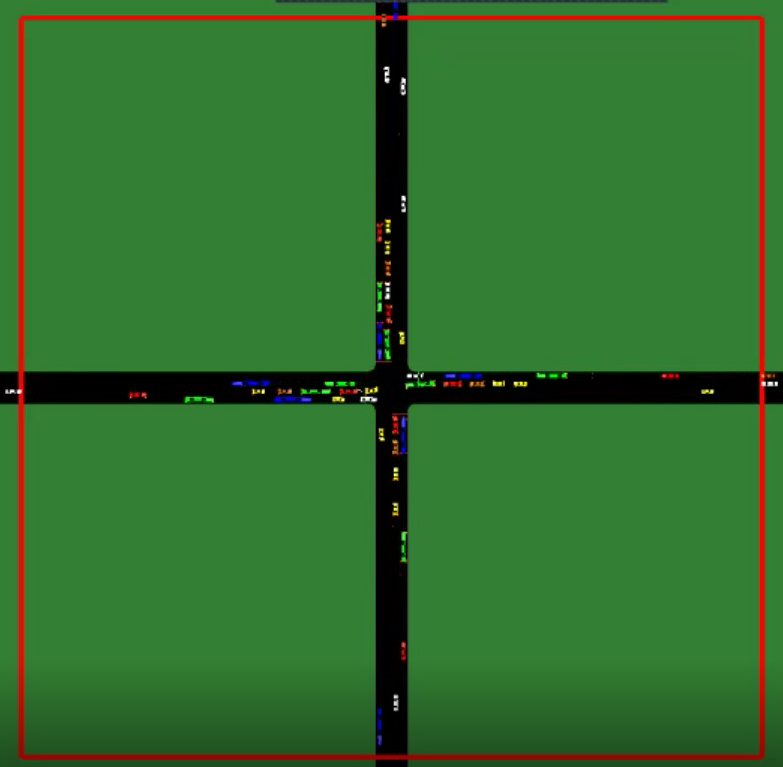
\includegraphics[width=\textwidth]{visuals/network/intersection_overview}
  \caption{Simulated four-way intersection with vehicles on all four
    approaches. The red bounding square marks the 300\,m$\times$300\,m in-box
    detection zone that defines the CO\textsubscript{2} scope
    (Eq.~\ref{eq:co2metric}).}
  \label{fig:intersection_overview}
\end{figure}

\begin{figure}[H]
  \centering
  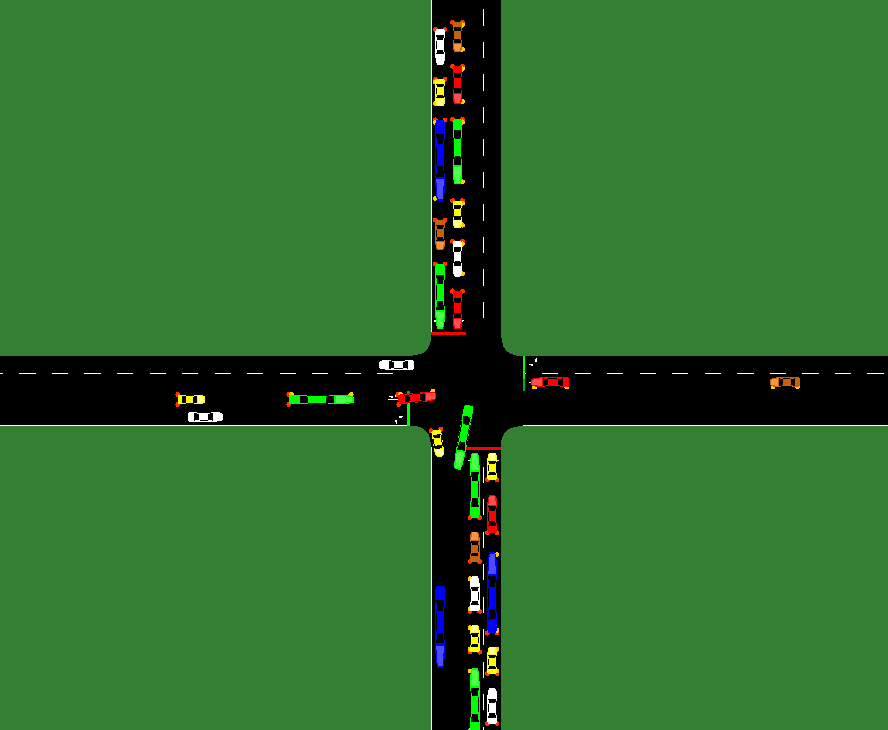
\includegraphics[width=0.75\textwidth]{visuals/network/intersection_zoomed}
  \caption{Close-up of the signal head and the in-box detection zone (red
    outline).}
  \label{fig:intersection_zoomed}
\end{figure}

The per-vehicle in-box CO\textsubscript{2} metric is:
\begin{equation}
  \text{CO}_2\text{/veh} =
    \frac{\displaystyle\sum_{t,\,v:\,\texttt{in\_box}(v,t)=\text{True}}
           \text{CO}_2(v,t)}
         {N_{\text{unique vehicles}}}
  \label{eq:co2metric}
\end{equation}
where $\text{CO}_2(v,t)$ is the instantaneous emission (mg) of vehicle $v$
at step $t$, summed over all steps during which that vehicle is inside the
detection zone, and $N_{\text{unique vehicles}}$ is the total distinct-vehicle
count in the run.

\subsection{Vehicle Fleet and Demand}
\label{sec:fleet}

The default fleet represents a mixed urban profile: Car Standard 40\%,
Bus City 15\%, Truck Light 15\%, Delivery Van 10\%, Vehicle General 10\%,
Coach Long 10\%. Each vehicle type is assigned SUMO's built-in HBEFA3
emission class. Demand is Poisson-distributed at a specified arrival rate
(veh/hr), and each simulation runs for 3\,600\,s with a 270\,s warm-up
period covering three signal cycles.

\subsection{Random Seeds}
\label{sec:seeds}

All experiments use ten seeds
$\mathcal{S}=\{5,10,13,17,25,37,42,50,75,77\}$ to control SUMO's internal
stochastic routing and gap-acceptance noise. Reported statistics are means
over $\mathcal{S}$ unless noted otherwise.

%% ============================================================
\section{Control Algorithms}
\label{sec:algo}

Both controllers share Rules 1--2 (minimum and maximum green bounds) and
differ only in Rule 3, the phase-termination criterion. SAC terminates on
traffic absence (gap $>$ MAX\_GAP); EBAC terminates on emission surplus
($\text{em\_red} - \text{em\_green} > \theta$). Both respond to the same
underlying phenomenon---a queue forming on the red approach---but EBAC
weights each vehicle by its current CO\textsubscript{2} rate rather than
counting vehicles uniformly, giving heavier high-emission vehicles implicit
priority.

\subsection{Standard Actuated Control (SAC)}

Algorithm~\ref{alg:sac} presents the SAC switch-decision logic evaluated at
each simulation step while a green phase is active. Parameters are
MIN\_GREEN\,=\,8\,s, MAX\_GREEN\,=\,60\,s, MAX\_GAP\,=\,3.0\,s.

\begin{algorithm}[H]
\caption{Standard Actuated Control (SAC) — switch decision}
\label{alg:sac}
\begin{algorithmic}[1]
\Require Current green phase $g$, phase duration $d$, TraCI edge queries
\Ensure \textsc{Boolean}: switch (\textbf{true}) or hold (\textbf{false})
\If{$d <$ MIN\_GREEN} \Return \textbf{false} \Comment{hold — minimum green not yet met}
\EndIf
\If{$d \geq$ MAX\_GREEN} \Return \textbf{true} \Comment{force switch — max green cap}
\EndIf
\ForAll{edge $e$ in GREEN\_PHASES$[g]$}
  \State $V_e \gets$ \Call{getLastStepVehicleIDs}{$e$}
  \If{$V_e = \emptyset$} \Return \textbf{true} \Comment{empty lane — gap detected}
  \EndIf
  \State $v_{\text{last}} \gets$ last vehicle in $V_e$
  \State $(tls, \_, \text{gap}) \gets$ \Call{getNextTLS}{$v_{\text{last}}$}
  \If{$\text{gap} >$ MAX\_GAP} \Return \textbf{true} \Comment{gap exceeds threshold}
  \EndIf
\EndFor
\State \Return \textbf{false} \Comment{hold green}
\end{algorithmic}
\end{algorithm}

\subsection{Emission-Based Actuated Control (EBAC)}

Algorithm~\ref{alg:ebac} retains Rules 1--2 from SAC and replaces Rule 3
with a real-time CO\textsubscript{2} comparison. The switch fires when the
aggregate emission rate on the opposing (red) approaches exceeds that on the
currently green approaches by more than the single tunable parameter
$\theta \equiv$ EMISSION\_THRESHOLD (mg/s).

\begin{algorithm}[H]
\caption{Emission-Based Actuated Control (EBAC) — switch decision}
\label{alg:ebac}
\begin{algorithmic}[1]
\Require Current green phase $g$, phase duration $d$, threshold $\theta$
\Ensure \textsc{Boolean}: switch (\textbf{true}) or hold (\textbf{false})
\If{$d <$ MIN\_GREEN} \Return \textbf{false}
\EndIf
\If{$d \geq$ MAX\_GREEN} \Return \textbf{true}
\EndIf
\State $g_{\text{opp}} \gets $ opposing phase of $g$ \Comment{$0 \leftrightarrow 2$ on a 4-phase intersection}
\State $\text{em}_{\text{green}} \gets \sum_{e \in \text{GREEN\_PHASES}[g]} \sum_{v \in V_e} $ \Call{getCO2Emission}{$v$}
\State $\text{em}_{\text{red}}   \gets \sum_{e \in \text{GREEN\_PHASES}[g_{\text{opp}}]} \sum_{v \in V_e} $ \Call{getCO2Emission}{$v$}
\If{$\text{em}_{\text{red}} > \text{em}_{\text{green}} + \theta$}
  \State \Return \textbf{true} \Comment{red side emitting more — switch}
\EndIf
\State \Return \textbf{false} \Comment{hold green}
\end{algorithmic}
\end{algorithm}

Queued vehicles idle at high emission rates, while vehicles already moving
emit considerably less due to reduced engine load. When the red-side queue
becomes sufficiently more polluting than the current green flow, EBAC clears
it first to reduce total intersection emissions. MIN\_GREEN/MAX\_GREEN bounds
remain identical to SAC, so the throughput impact of any single switch is
bounded by the same envelope.

%% ============================================================
\section{Capacity Analysis and Regime Classification}
\label{sec:capacity}

Before the threshold search, we characterised intersection capacity to
select representative demand levels spanning the full congestion range.
Demand was swept from 500 to 7\,500\,veh/hr in 100-unit steps; at each
level, ten seeds were run and the mean maximum discharge per cycle was
recorded. The signal cycle is 90\,s.

\begin{figure}[H]
  \centering
  \includegraphics[width=\textwidth]%
    {visuals/capacity_plots/01_discharge_vs_demand}
  \caption{Per-cycle vehicle discharge as a function of demand
    (90\,s cycle; 71 volumes, 10 seeds). Blue line/band: mean max discharge
    ($\pm$1\,SD); orange line/band: mean average discharge. Red dashed line:
    estimated capacity of 97\,veh/cycle ($\approx$3\,880\,veh/hr). Purple dotted
    line: critical volume at $V=7\,400$\,veh/hr, where the plateau detector
    confirms saturation.}
  \label{fig:discharge}
\end{figure}

\begin{figure}[H]
  \centering
  \includegraphics[width=\textwidth]%
    {visuals/capacity_plots/03a_vc_per_cycle_bars_with_los}
  \caption{Per-cycle $v/c$ ratio by demand, split into three contiguous
    vertical panels. Bar colors encode an HCM-style level-of-service proxy
    derived from $v/c$ (A~$<$35\%; B~35--55\%; C~55--75\%; D~75--90\%;
    E~90--100\%; F~$>$100\%); capacity is 97\,veh/cycle. LOS shown here is a
    $v/c$ proxy, not delay-based HCM LOS~\cite{TRB2000HCM}.}
  \label{fig:vc_bars}
\end{figure}

\begin{figure}[H]
  \centering
  \includegraphics[width=\textwidth]%
    {visuals/capacity_plots/04_capacity_dashboard}
  \caption{Capacity dashboard: (a) discharge/cycle with capacity line;
    (b) marginal discharge gain per +100\,veh/hr demand step; (c) per-cycle
    $v/c$ with LOS-proxy bands. Confirms plateau onset at
    $V=7\,400$\,veh/hr; the four representative regimes in
    Table~\ref{tab:los} are drawn from within this envelope.}
  \label{fig:cap_dashboard}
\end{figure}

Table~\ref{tab:los} lists the four representative volumes classified by
Level-of-Service~\cite{TRB2000HCM}. Worth noting is the sharp jump in
baseline CO\textsubscript{2}/veh from Near-saturation (315\,284\,mg) to
Breakdown onset (511\,004\,mg)---an increase of nearly 62\%. This reflects
queue spillback: vehicles on red approaches idle through significantly more
cycles, substantially inflating per-vehicle emissions and creating the
asymmetry EBAC is designed to exploit.

\begin{table}[H]
  \centering
  \caption{Representative volumes and Level-of-Service classification.}
  \label{tab:los}
  \begin{tabular}{lcccc}
    \toprule
    \textbf{Regime} & \textbf{Volume} & \textbf{$v/c$ (\%)} &
    \textbf{LOS} & \textbf{Baseline CO$_2$/veh (mg)} \\
    \midrule
    Free-flow       & 1\,500 & 38.9 & B & 269\,033 \\
    Near-saturation & 2\,900 & 74.7 & C & 315\,284 \\
    Breakdown onset & 3\,300 & 82.9 & D & 511\,004 \\
    Gridlock        & 5\,000 & 91.1 & E & 717\,416 \\
    \bottomrule
  \end{tabular}
\end{table}

%% ============================================================
\section{Experiment 1: Constrained Exhaustive Grid Search}
\label{sec:exp1}

\subsection{Design}

EMISSION\_THRESHOLD was searched over 50 values in [10, 300]\,mg/s: a
coarse grid of 42 globally distributed points followed by fine-grid
refinement of 8 values around per-regime coarse optima ($\pm 1$ bracket).
Every combination of threshold~$\times$~volume~$\times$~seed was simulated
(50~$\times$~4~$\times$~10~=~2\,000 runs). A candidate threshold is
\emph{valid} only when its mean throughput change versus baseline exceeds
$-1\%$; the valid threshold with the highest mean in-box
CO\textsubscript{2} saving is declared optimal. $\text{thr}=50$\,mg/s is
treated as a pre-specified reference for the statistical tests, since it was
fixed before the search began. Of the 200 threshold--regime combinations,
only three violated the constraint: $\text{thr}=32$ at V2900
($\Delta\text{tput}=-2.44\%$) and $\text{thr}=\{21,27\}$ at V5000
($-2.15\%$ and $-3.42\%$).

\begin{figure}[H]
  \centering
  \includegraphics[width=\textwidth]%
    {experiments/threshold_search/visuals/co2_vs_threshold_by_regime}
  \caption{In-box CO$_2$ savings (\%, coloured line, left axis) and throughput
    change (\%, grey triangles, right axis) versus emission threshold, per
    regime. Green bands mark the sweet spot (CO$_2>0$ AND
    $\Delta\text{tput}>-1\%$); dashed green line marks the throughput-constrained
    optimum. Optima: 41, 42, 135, 138\,mg/s for the four regimes.}
  \label{fig:co2_vs_thr}
\end{figure}

\begin{figure}[H]
  \centering
  \includegraphics[width=\textwidth]%
    {experiments/threshold_search/visuals/stable_region_analysis}
  \caption{Stable-threshold regions per regime (rolling mean $\pm$0.3\% band;
    plateau where rolling $\geq$ peak$-0.3$\%; optimum = max CO$_2$ saving with
    $\Delta\text{tput}>-1\%$). Peak savings 0.37, 1.95, 3.01, 0.20\% for the
    four regimes.}
  \label{fig:stable}
\end{figure}

\begin{figure}[H]
  \centering
  \includegraphics[width=0.85\textwidth]%
    {experiments/threshold_search/visuals/optimal_threshold_by_regime}
  \caption{Constrained-optimum threshold per regime, annotated with peak
    CO$_2$ savings. The optimum roughly doubles between under-saturated
    ($\sim$40\,mg/s) and saturated ($\sim$135--140\,mg/s) regimes.}
  \label{fig:opt_thr}
\end{figure}

\subsection{Results}

Table~\ref{tab:optimal} summarises the constrained-optimum results.

\begin{table}[H]
  \centering
  \caption{Constrained-optimum threshold results (in-box CO$_2$, 10 seeds per
  cell). Note that throughput is preserved exactly in every regime.}
  \label{tab:optimal}
  \begin{tabular}{lcccc}
    \toprule
    \textbf{Regime} & \textbf{Opt. thr} &
    \textbf{$\Delta$CO$_2$ (\%)} & \textbf{$\Delta$Tput (\%)} & \textbf{$\Delta$Wait (\%)} \\
    \midrule
    Free-flow (V1500)       & 41  & $+0.37$ & $0.00$ & $-4.52$ \\
    Near-saturation (V2900) & 42  & $+1.95$ & $0.00$ & $-8.66$ \\
    Breakdown onset (V3300) & 135 & $+3.01$ & $0.00$ & $-13.58$ \\
    Gridlock (V5000)        & 138 & $+0.20$ & $0.00$ & $-14.99$ \\
    \bottomrule
  \end{tabular}
\end{table}

Four patterns stand out in these results. All four regimes preserve
throughput exactly at their optimal threshold ($\Delta\text{tput}=0.00\%$),
showing that emission reduction and throughput preservation are not in
conflict at moderate-to-high congestion when the threshold is properly
calibrated. Wait time falls in every regime---ranging from $-4.5\%$ to
$-15.0\%$---a co-benefit not seen with the gap-based baseline: EBAC clears
high-emission queues earlier, so all vehicles benefit even when their own
emissions are low. The optimal threshold itself grows with congestion (41
vs 42 vs 135 vs 138\,mg/s), which is consistent with the rising absolute
emission rates in Table~\ref{tab:los}. Perhaps most striking, Breakdown
onset shows the largest CO\textsubscript{2} gain ($+3.01\%$), and this
coincides precisely with the sharpest per-vehicle emission jump in the
dataset---an alignment that suggests the two phenomena share the same
underlying cause.

\subsection{Statistical Significance}
\label{sec:stats}

Two paired tests were applied: an unpaired Welch $t$-test (unequal
variance) and a paired $t$-test exploiting the matched-seed design, which
is more powerful. Tests were performed at the pre-specified
$\text{thr}=50$ and at each regime-specific optimal threshold (the latter
carries a mild selection-bias caution).

\begin{table}[H]
  \centering
  \caption{Statistical test results (CO$_2$/veh, 10 seeds).}
  \label{tab:stats}
  \begin{tabular}{llcccc}
    \toprule
    \textbf{Regime} & \textbf{Thr} & \textbf{Mean sav.} &
    \textbf{Paired $p$} & \textbf{Cohen's $d$} & \textbf{Sig.} \\
    \midrule
    \multirow{2}{*}{Free-flow}
      & 50   & $-0.37\%$ & 0.251 & 0.56 & n.s. \\
      & 41*  & $+0.37\%$ & 0.183 & 0.65 & n.s. \\[3pt]
    \multirow{2}{*}{Near-sat.}
      & 50   & $+1.33\%$ & \textbf{0.045} & 1.19 & * \\
      & 42*  & $+1.90\%$ & \textbf{0.007} & 1.67 & ** \\[3pt]
    \multirow{2}{*}{Breakdown}
      & 50   & $+1.27\%$ & 0.249 & 0.53 & n.s. \\
      & 135* & $+2.84\%$ & \textbf{0.038} & 1.14 & * \\[3pt]
    \multirow{2}{*}{Gridlock}
      & 50   & $-0.26\%$ & 0.065 & 0.58 & n.s. \\
      & 138* & $+0.19\%$ & 0.374 & 0.43 & n.s. \\
    \bottomrule
    \multicolumn{6}{l}{\footnotesize * Post-hoc optimal threshold; significance may be optimistic.} \\
    \multicolumn{6}{l}{\footnotesize ** $p<0.01$;\ * $p<0.05$;\ n.s. $p\geq 0.05$;\ $d\geq 0.8$ = large effect.} \\
  \end{tabular}
\end{table}

The pre-specified $\text{thr}=50$ test serves as the most conservative
benchmark. Near-saturation is the only regime where it reaches significance
($p=0.045$, $d=1.19$), which confirms that the EBAC effect at V2900 is
real---not an artefact of threshold selection. Effect sizes at the post-hoc
optimal threshold are large ($d>0.8$) for both Near-saturation and
Breakdown onset, indicating practically meaningful savings even where
$p$-values alone would be borderline with $n=10$. Gridlock tells a
different story: consistently near-zero or slightly negative savings, because
at full saturation both approaches are saturated and the asymmetry EBAC
depends on largely disappears.

\subsection{Stable-Region Analysis and Universal Threshold}
\label{sec:stable}

Fig.~\ref{fig:stable} overlays a 5-point centred rolling average on each
threshold scan. Free-flow and Near-saturation both exhibit broad plateaus
centred around 20--50\,mg/s. Breakdown onset has a narrower plateau around
120--140\,mg/s. Gridlock shows no discernible plateau at all, consistent
with the statistical null across the full grid. For deployments without
per-regime calibration, $\text{thr}=44$\,mg/s lies within the stable
plateau for both Free-flow and Near-saturation, and its Breakdown-onset
result ($+1.74\%$) is only modestly below the regime optimum ($+3.01\%$).
Table~\ref{tab:universal} compares.

\begin{table}[H]
  \centering
  \caption{Universal threshold thr$=44$\,mg/s vs.\ regime-specific optima.}
  \label{tab:universal}
  \begin{tabular}{lcc}
    \toprule
    \textbf{Regime} & \textbf{thr$=44$ savings} & \textbf{Optimal savings} \\
    \midrule
    Free-flow (V1500)       & $+0.34\%$ & $+0.37\%$ \\
    Near-saturation (V2900) & $+1.64\%$ & $+1.95\%$ \\
    Breakdown onset (V3300) & $+1.74\%$ & $+3.01\%$ \\
    Gridlock (V5000)        & $-0.03\%$ & $+0.20\%$ \\
    \bottomrule
  \end{tabular}
\end{table}

$\text{thr}=44$ is positive in three of four regimes and essentially neutral
at Gridlock ($-0.03\%$, within stochastic noise). It is recommended as a
deployable default pending real-world calibration.

\subsection{Consolidated Operational-Metric Summary}
\label{sec:opmetrics}

Reviewers of practical deployment work will reasonably ask whether emission
savings are ``paid for'' in operational terms. Table~\ref{tab:opmetrics}
consolidates every operational quantity at the constrained optimum. Across
all four regimes, EBAC delivers simultaneous CO\textsubscript{2} savings and
wait-time reductions, with throughput, speed, and travel time either
preserved or improved. No operational metric degrades under EBAC at the
throughput-constrained optimum.

\begin{table}[H]
  \centering
  \caption{Operational-metric summary at the constrained-optimum threshold.
    All values are percent change of EBAC vs.\ SAC baseline (positive = EBAC
    better where higher is better; positive $\Delta$CO$_2$ = saving; negative
    $\Delta$Wait/Travel = improvement).}
  \label{tab:opmetrics}
  \small
  \begin{tabularx}{\textwidth}{lcccccc}
    \toprule
    \textbf{Regime} & \textbf{Thr} & \textbf{$\Delta$CO$_2$} &
    \textbf{$\Delta$Tput} & \textbf{$\Delta$Speed} & \textbf{$\Delta$Travel} &
    \textbf{$\Delta$Wait} \\
    \midrule
    Free-flow       & 41  & $+0.37\%$ & $0.00\%$ & $+0.5\%$ & $-0.4\%$ & $-4.5\%$ \\
    Near-saturation & 42  & $+1.95\%$ & $0.00\%$ & $+0.8\%$ & $-1.9\%$ & $-8.7\%$ \\
    Breakdown onset & 135 & $+3.01\%$ & $0.00\%$ & $+0.1\%$ & $-0.7\%$ & $-13.6\%$ \\
    Gridlock        & 138 & $+0.20\%$ & $0.00\%$ & $-0.1\%$ & $+0.1\%$ & $-15.0\%$ \\
    \bottomrule
  \end{tabularx}
\end{table}

Queue-length data (measured as the mean number of stopped vehicles inside
the in-box zone) mirrors the wait-time trend. EBAC reduces the mean in-box
queue by 1--4 vehicles at Near-saturation and Breakdown onset, and by up to
7 vehicles at Gridlock. This is unsurprising in retrospect: queue length
correlates directly with the observed CO\textsubscript{2} rate, so the two
metrics move together by construction.

%% ============================================================
\section{Per-Regime Controller Comparison}
\label{sec:perregime}

We now decompose the aggregated results by regime, focusing on the
seed-level distributions that underlie each row of
Table~\ref{tab:optimal}. Each regime is represented by three panels: a
boxplot of the CO\textsubscript{2} distribution, a paired-seed line plot
revealing per-seed effect direction, and a grouped-bar plot of the in-box
and full-trip wait times.

\clearpage
\subsection{Free-Flow (V1500)}

\begin{figure}[H]
  \centering
  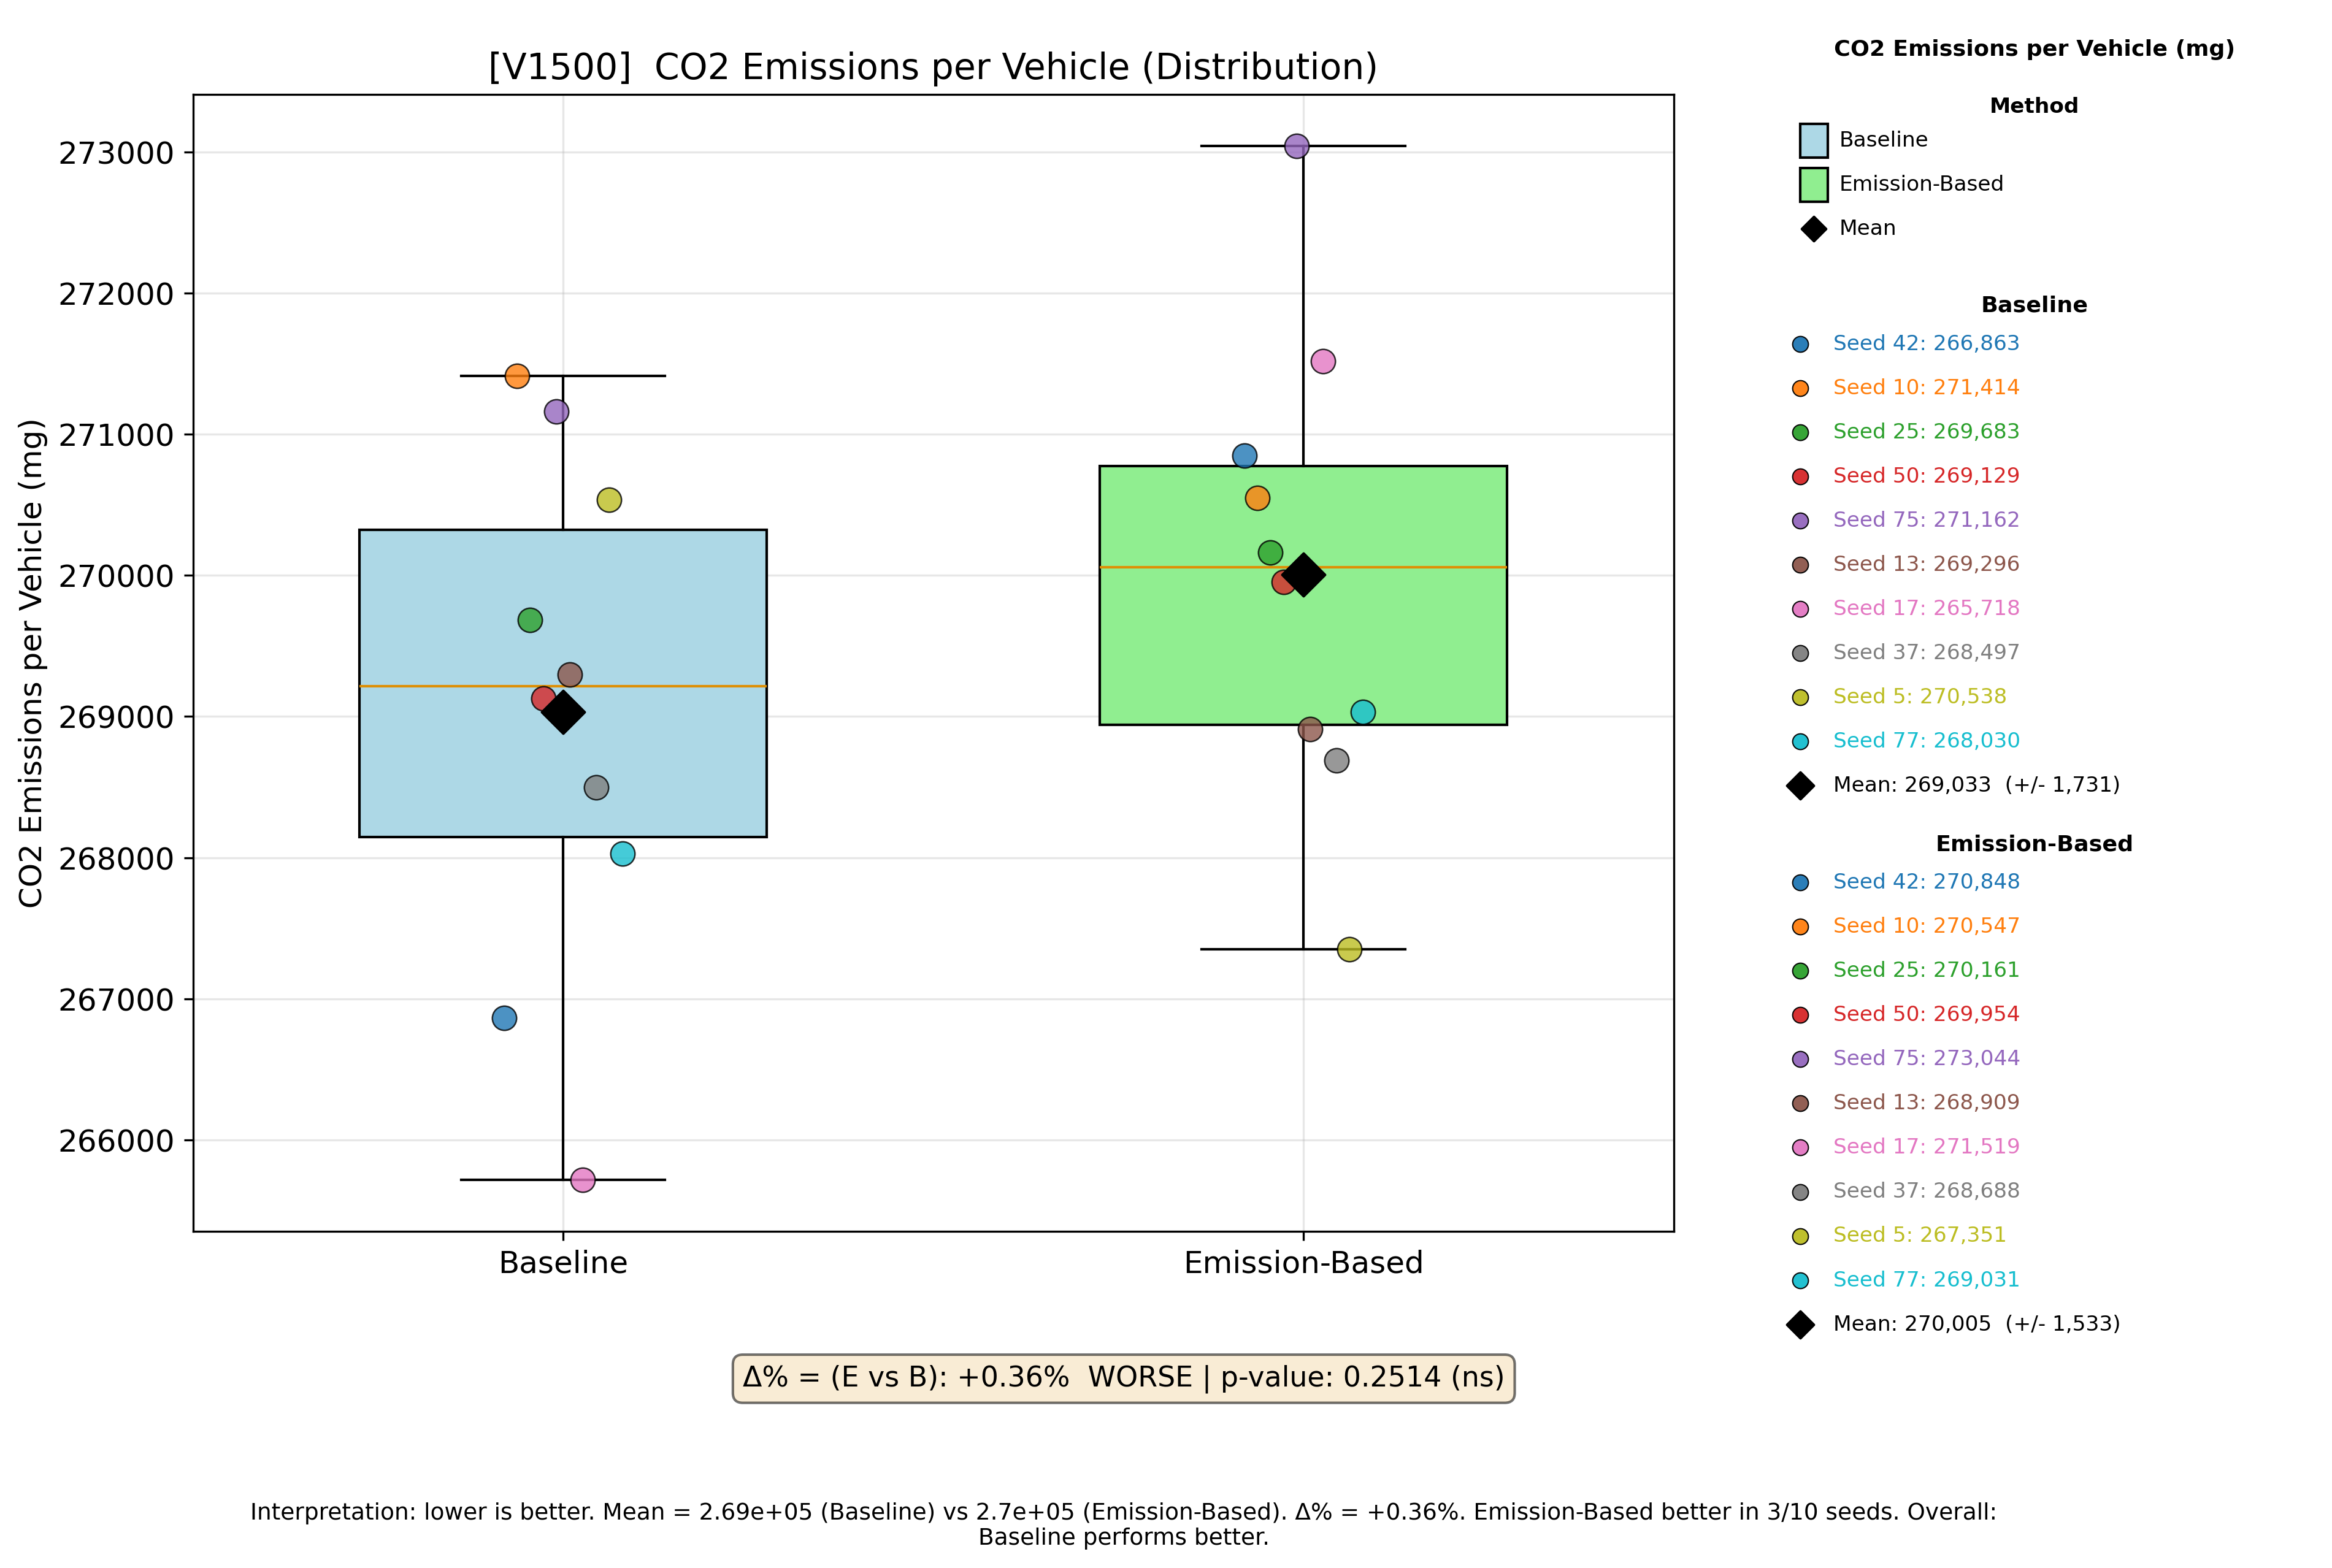
\includegraphics[width=0.85\textwidth]{visuals/V1500/single_boxplot_avg_co2_per_vehicle}
  \caption{V1500 (Free-flow) CO$_2$/vehicle distribution: baseline (blue) vs.
    emission-aware (green). At the reference threshold $\text{thr}=50$ the
    controllers are indistinguishable (paired $p=0.25$, 3/10 seeds).}
  \label{fig:v1500_box}
\end{figure}

\begin{figure}[H]
  \centering
  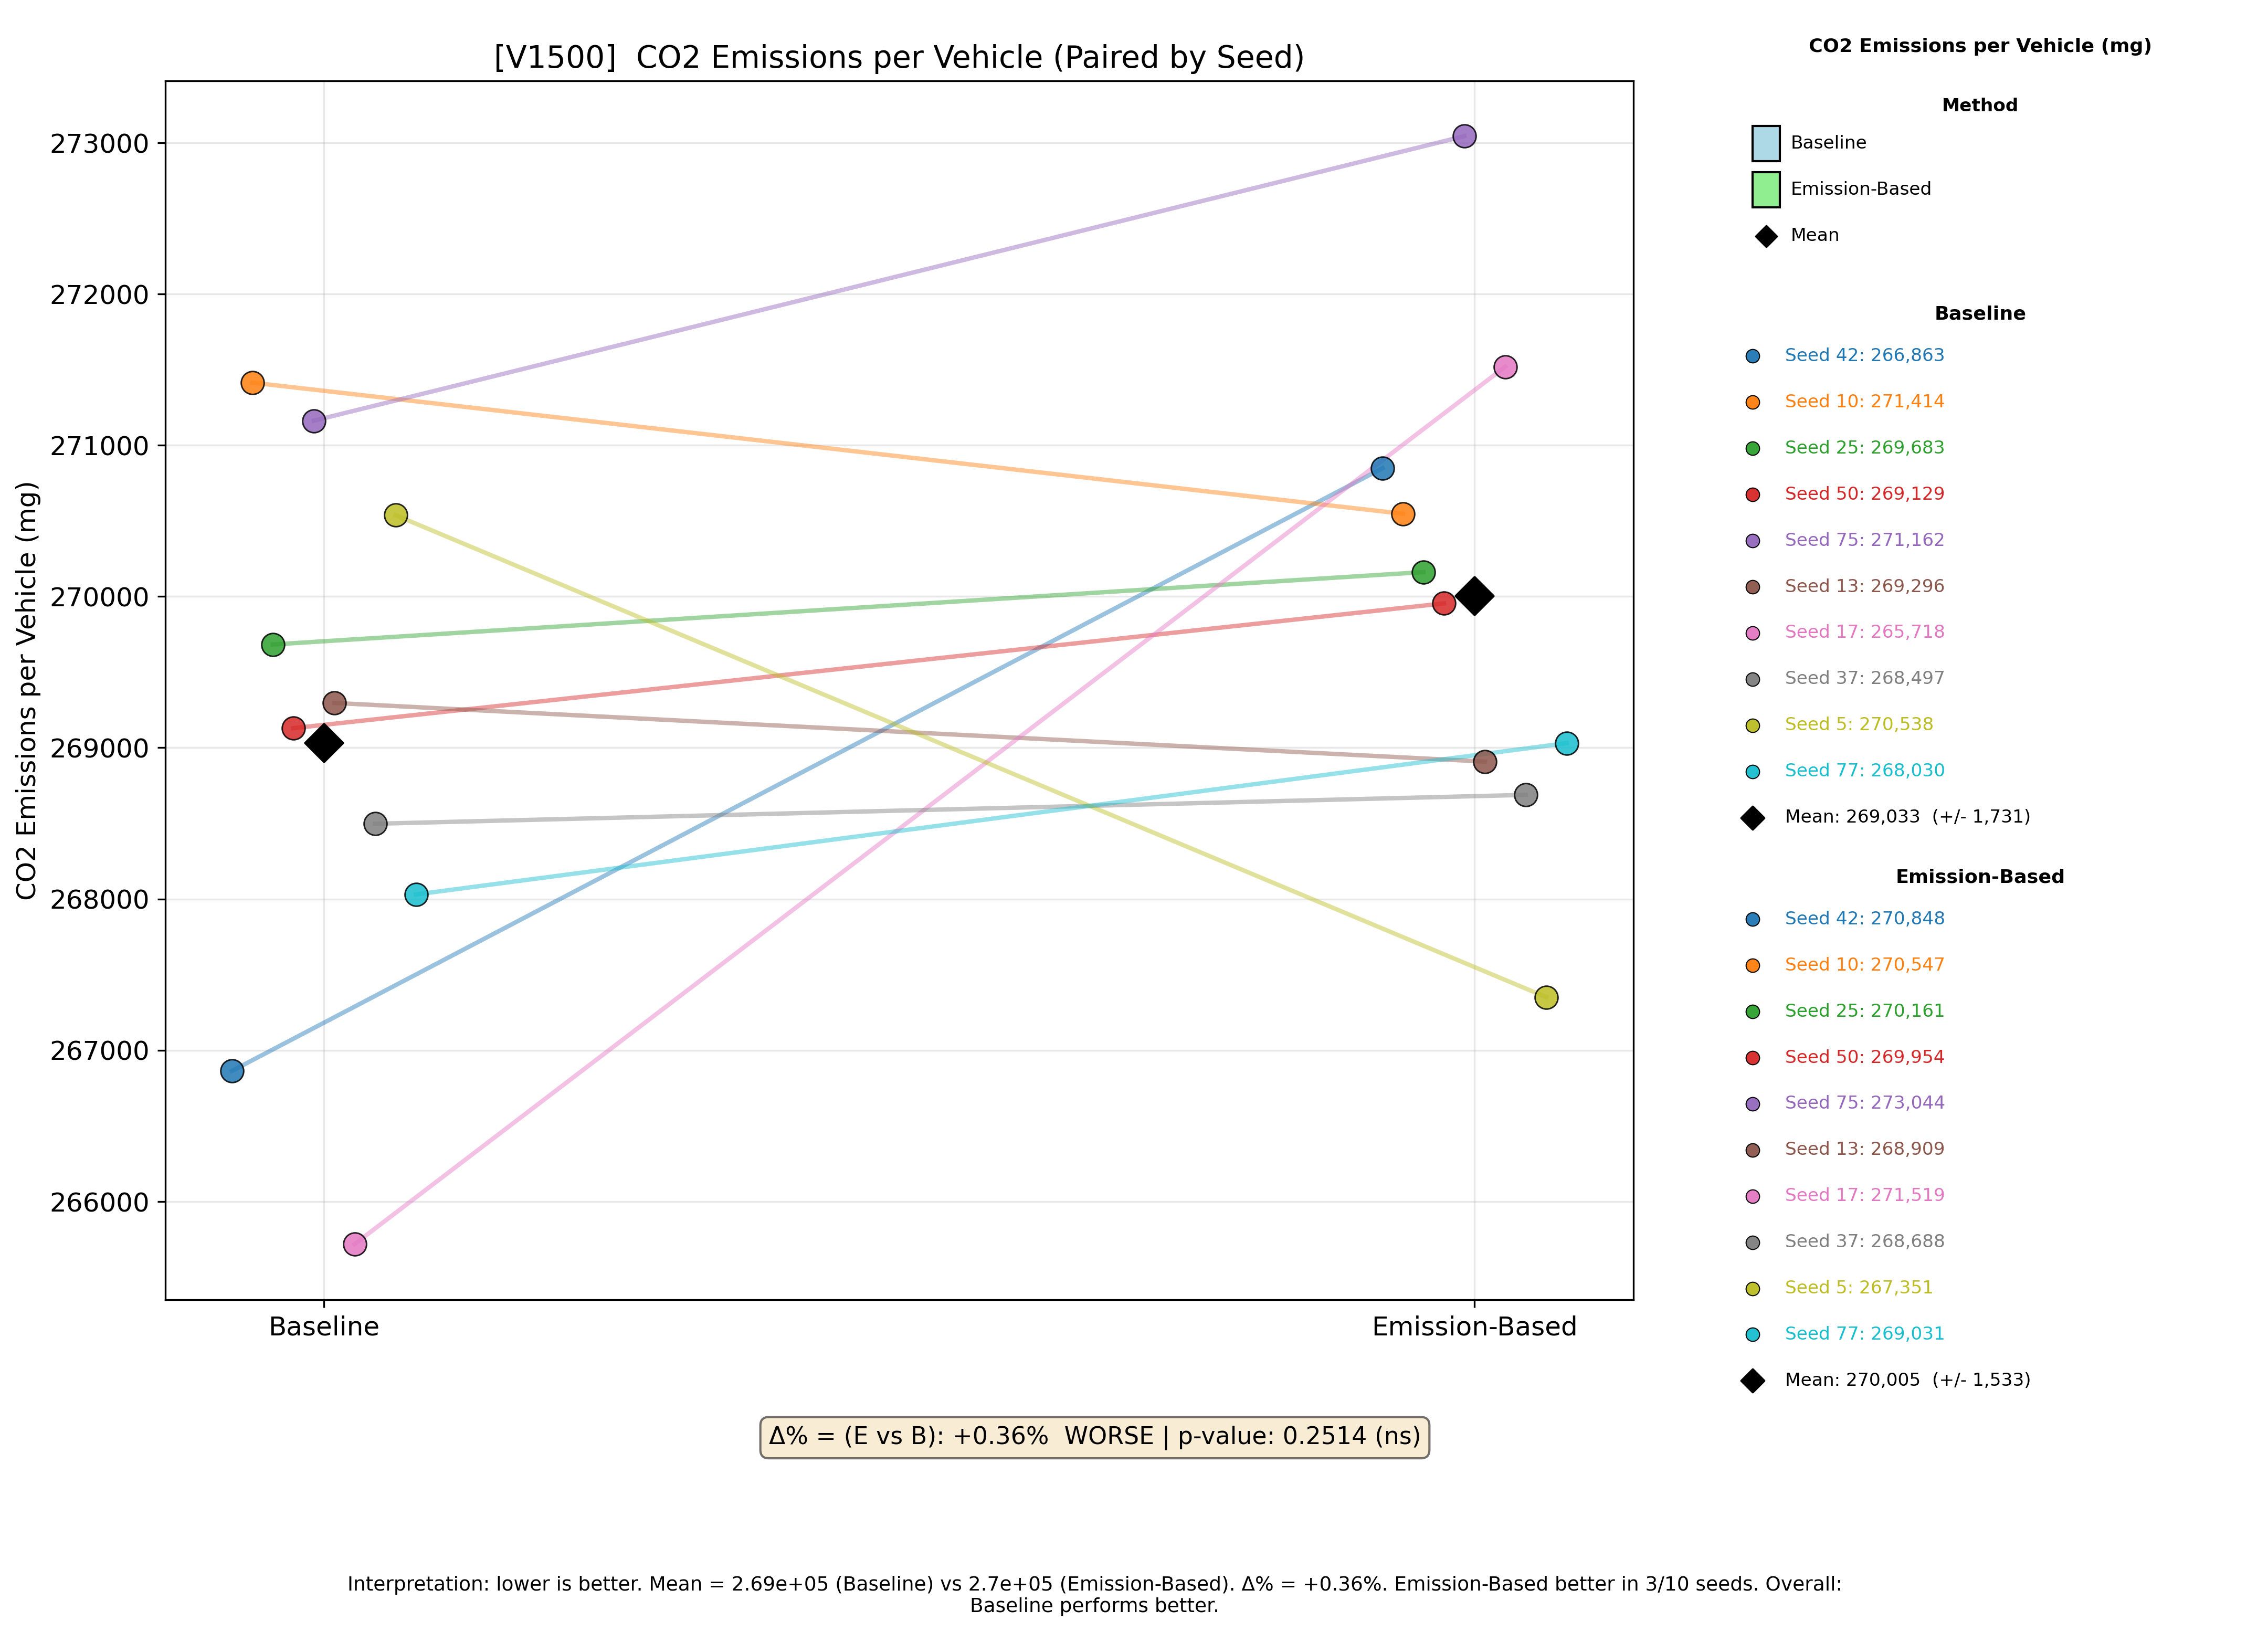
\includegraphics[width=0.85\textwidth]{visuals/V1500/single_paired_avg_co2_per_vehicle}
  \caption{V1500 paired-seed CO$_2$/vehicle comparison. Mixed line slopes reflect
    the small emission asymmetry available at $v/c=38.9\%$.}
  \label{fig:v1500_paired}
\end{figure}

\begin{figure}[H]
  \centering
  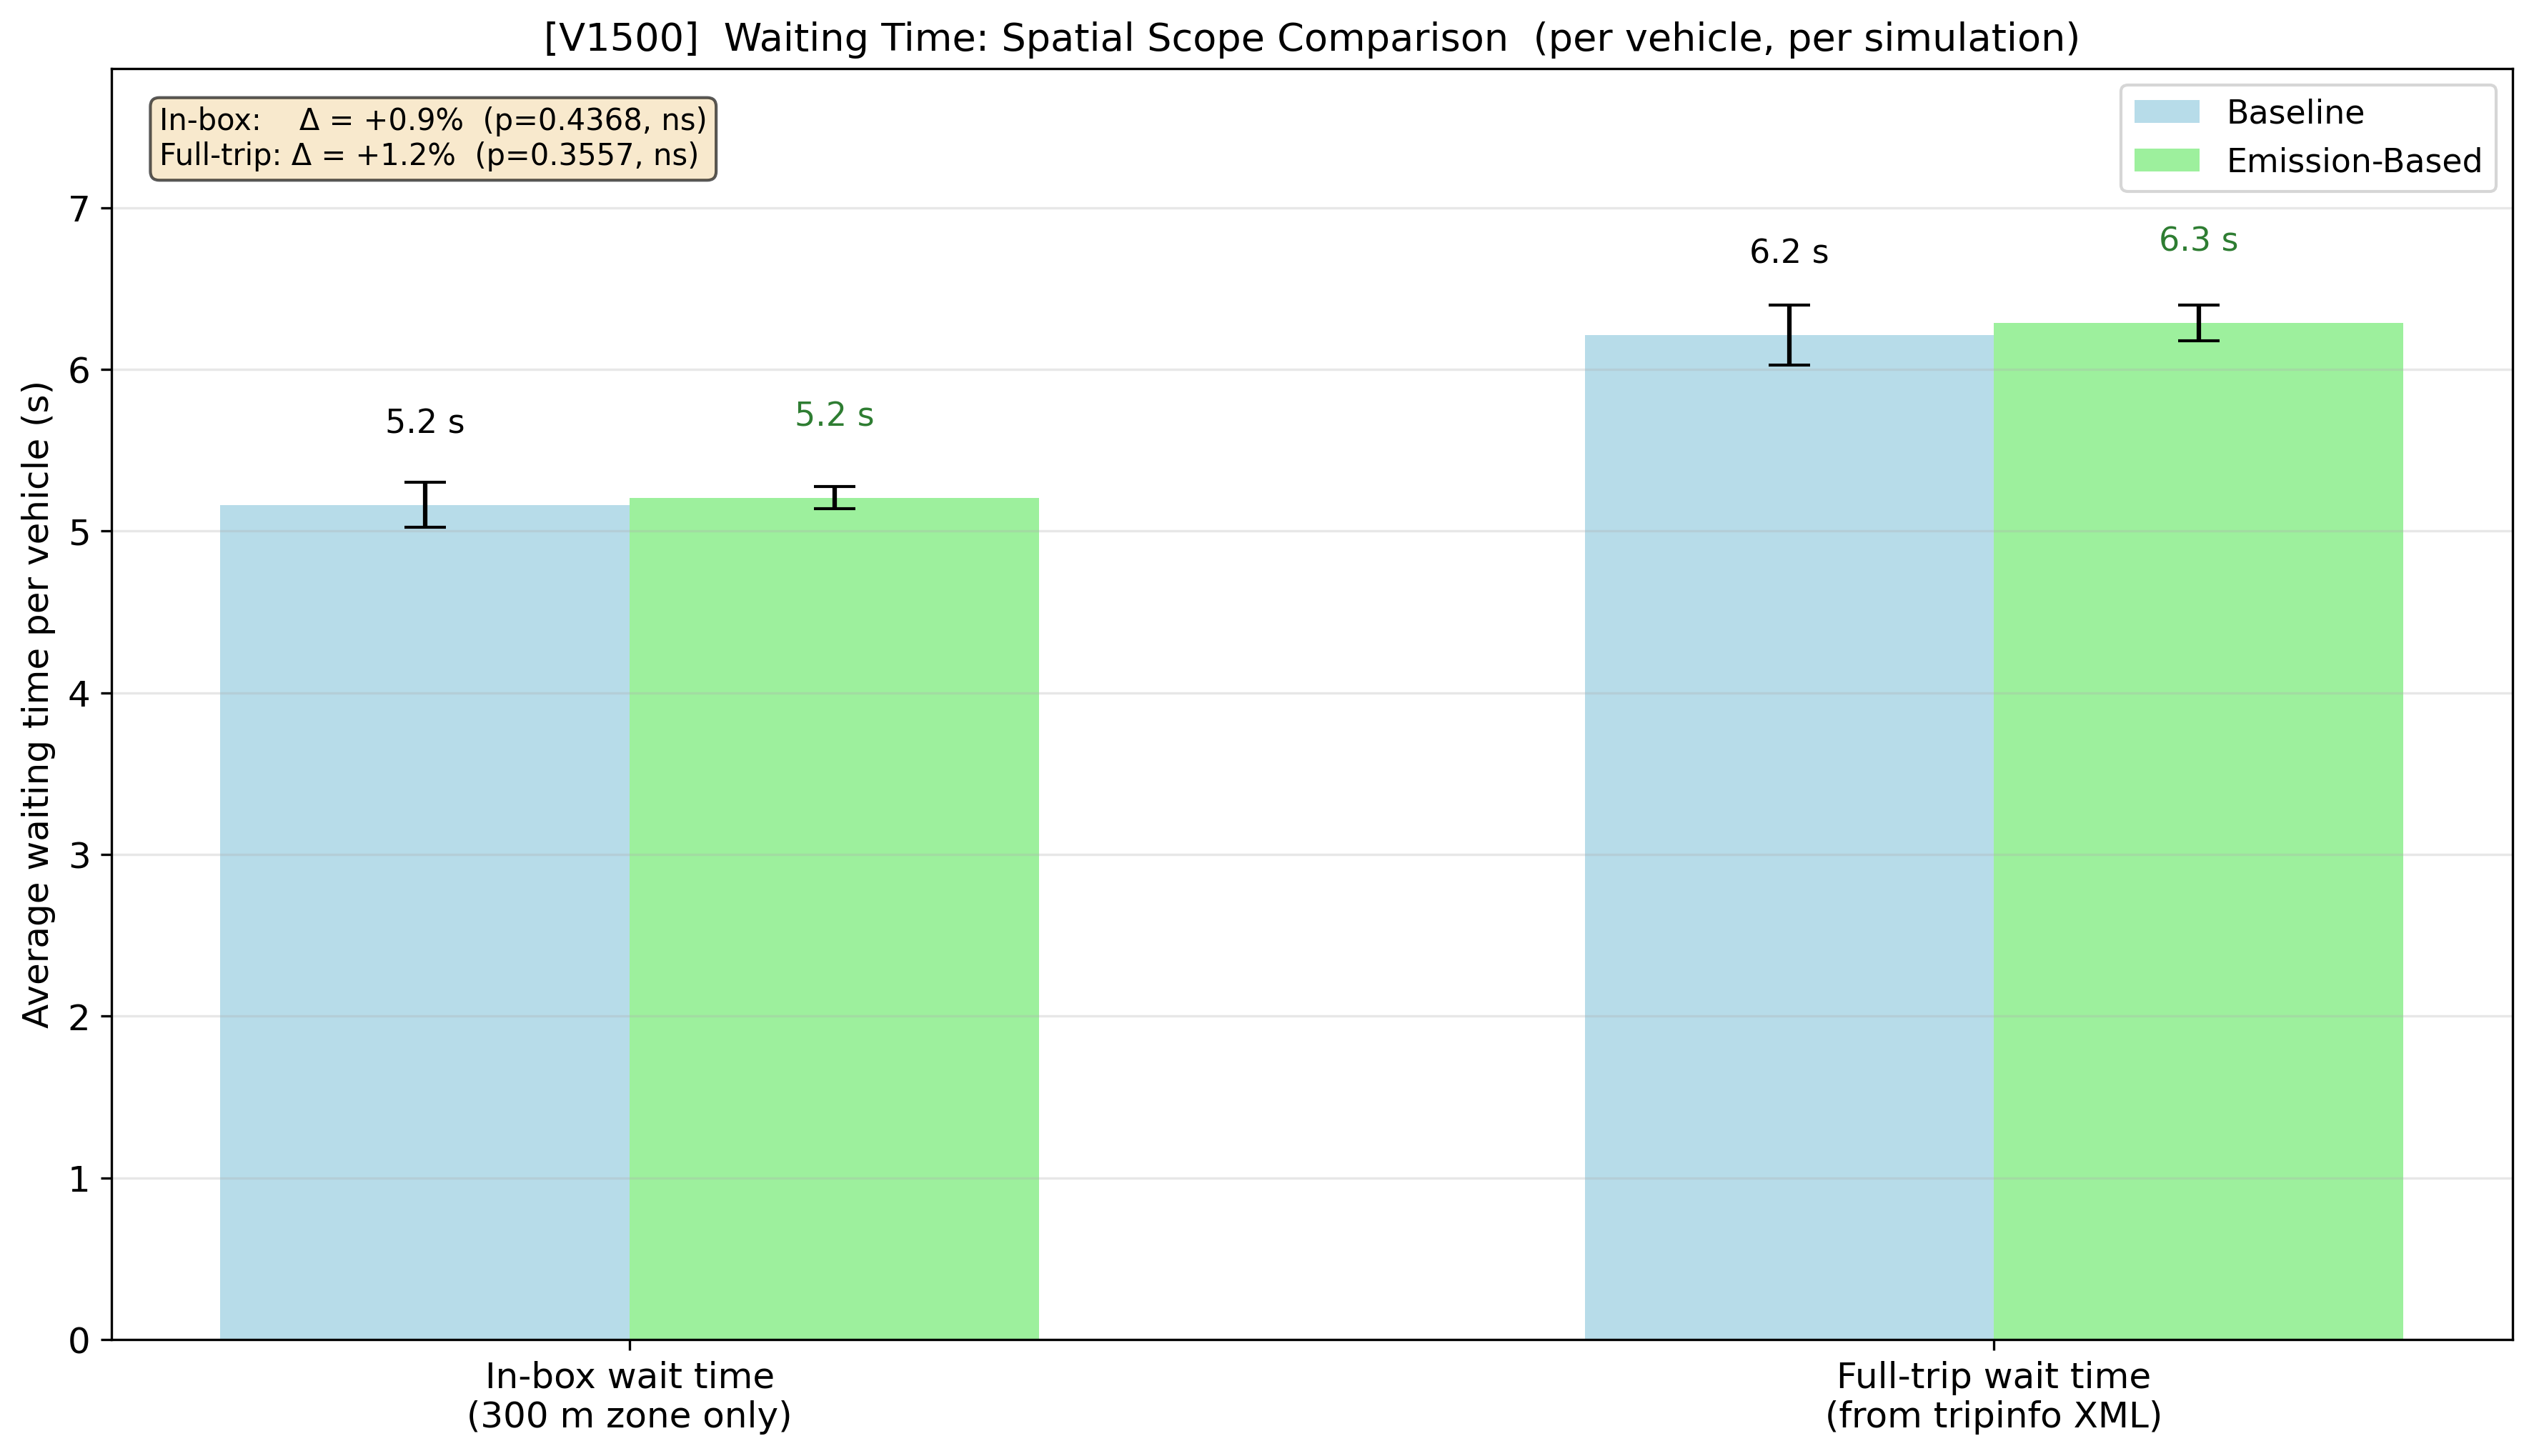
\includegraphics[width=0.85\textwidth]{visuals/V1500/dual_wait_time_comparison}
  \caption{V1500 in-box vs. full-trip wait, by seed. Both wait types are nearly
    identical between controllers ($\sim$5.2\,s in-box, $\sim$6.3\,s full-trip);
    the $\sim$1\,s gap is approach-lane wait, minimal at free-flow.}
  \label{fig:v1500_dw}
\end{figure}

At low demand ($v/c=38.9\%$), vehicles pass through with minimal queuing
under both strategies---the emission asymmetry EBAC exploits simply isn't
there. Wait time does fall by $2.2\%$, which suggests EBAC occasionally
clears small red-approach queues slightly earlier than gap detection would,
even at free-flow conditions.

\clearpage
\subsection{Near-Saturation (V2900)}

\begin{figure}[H]
  \centering
  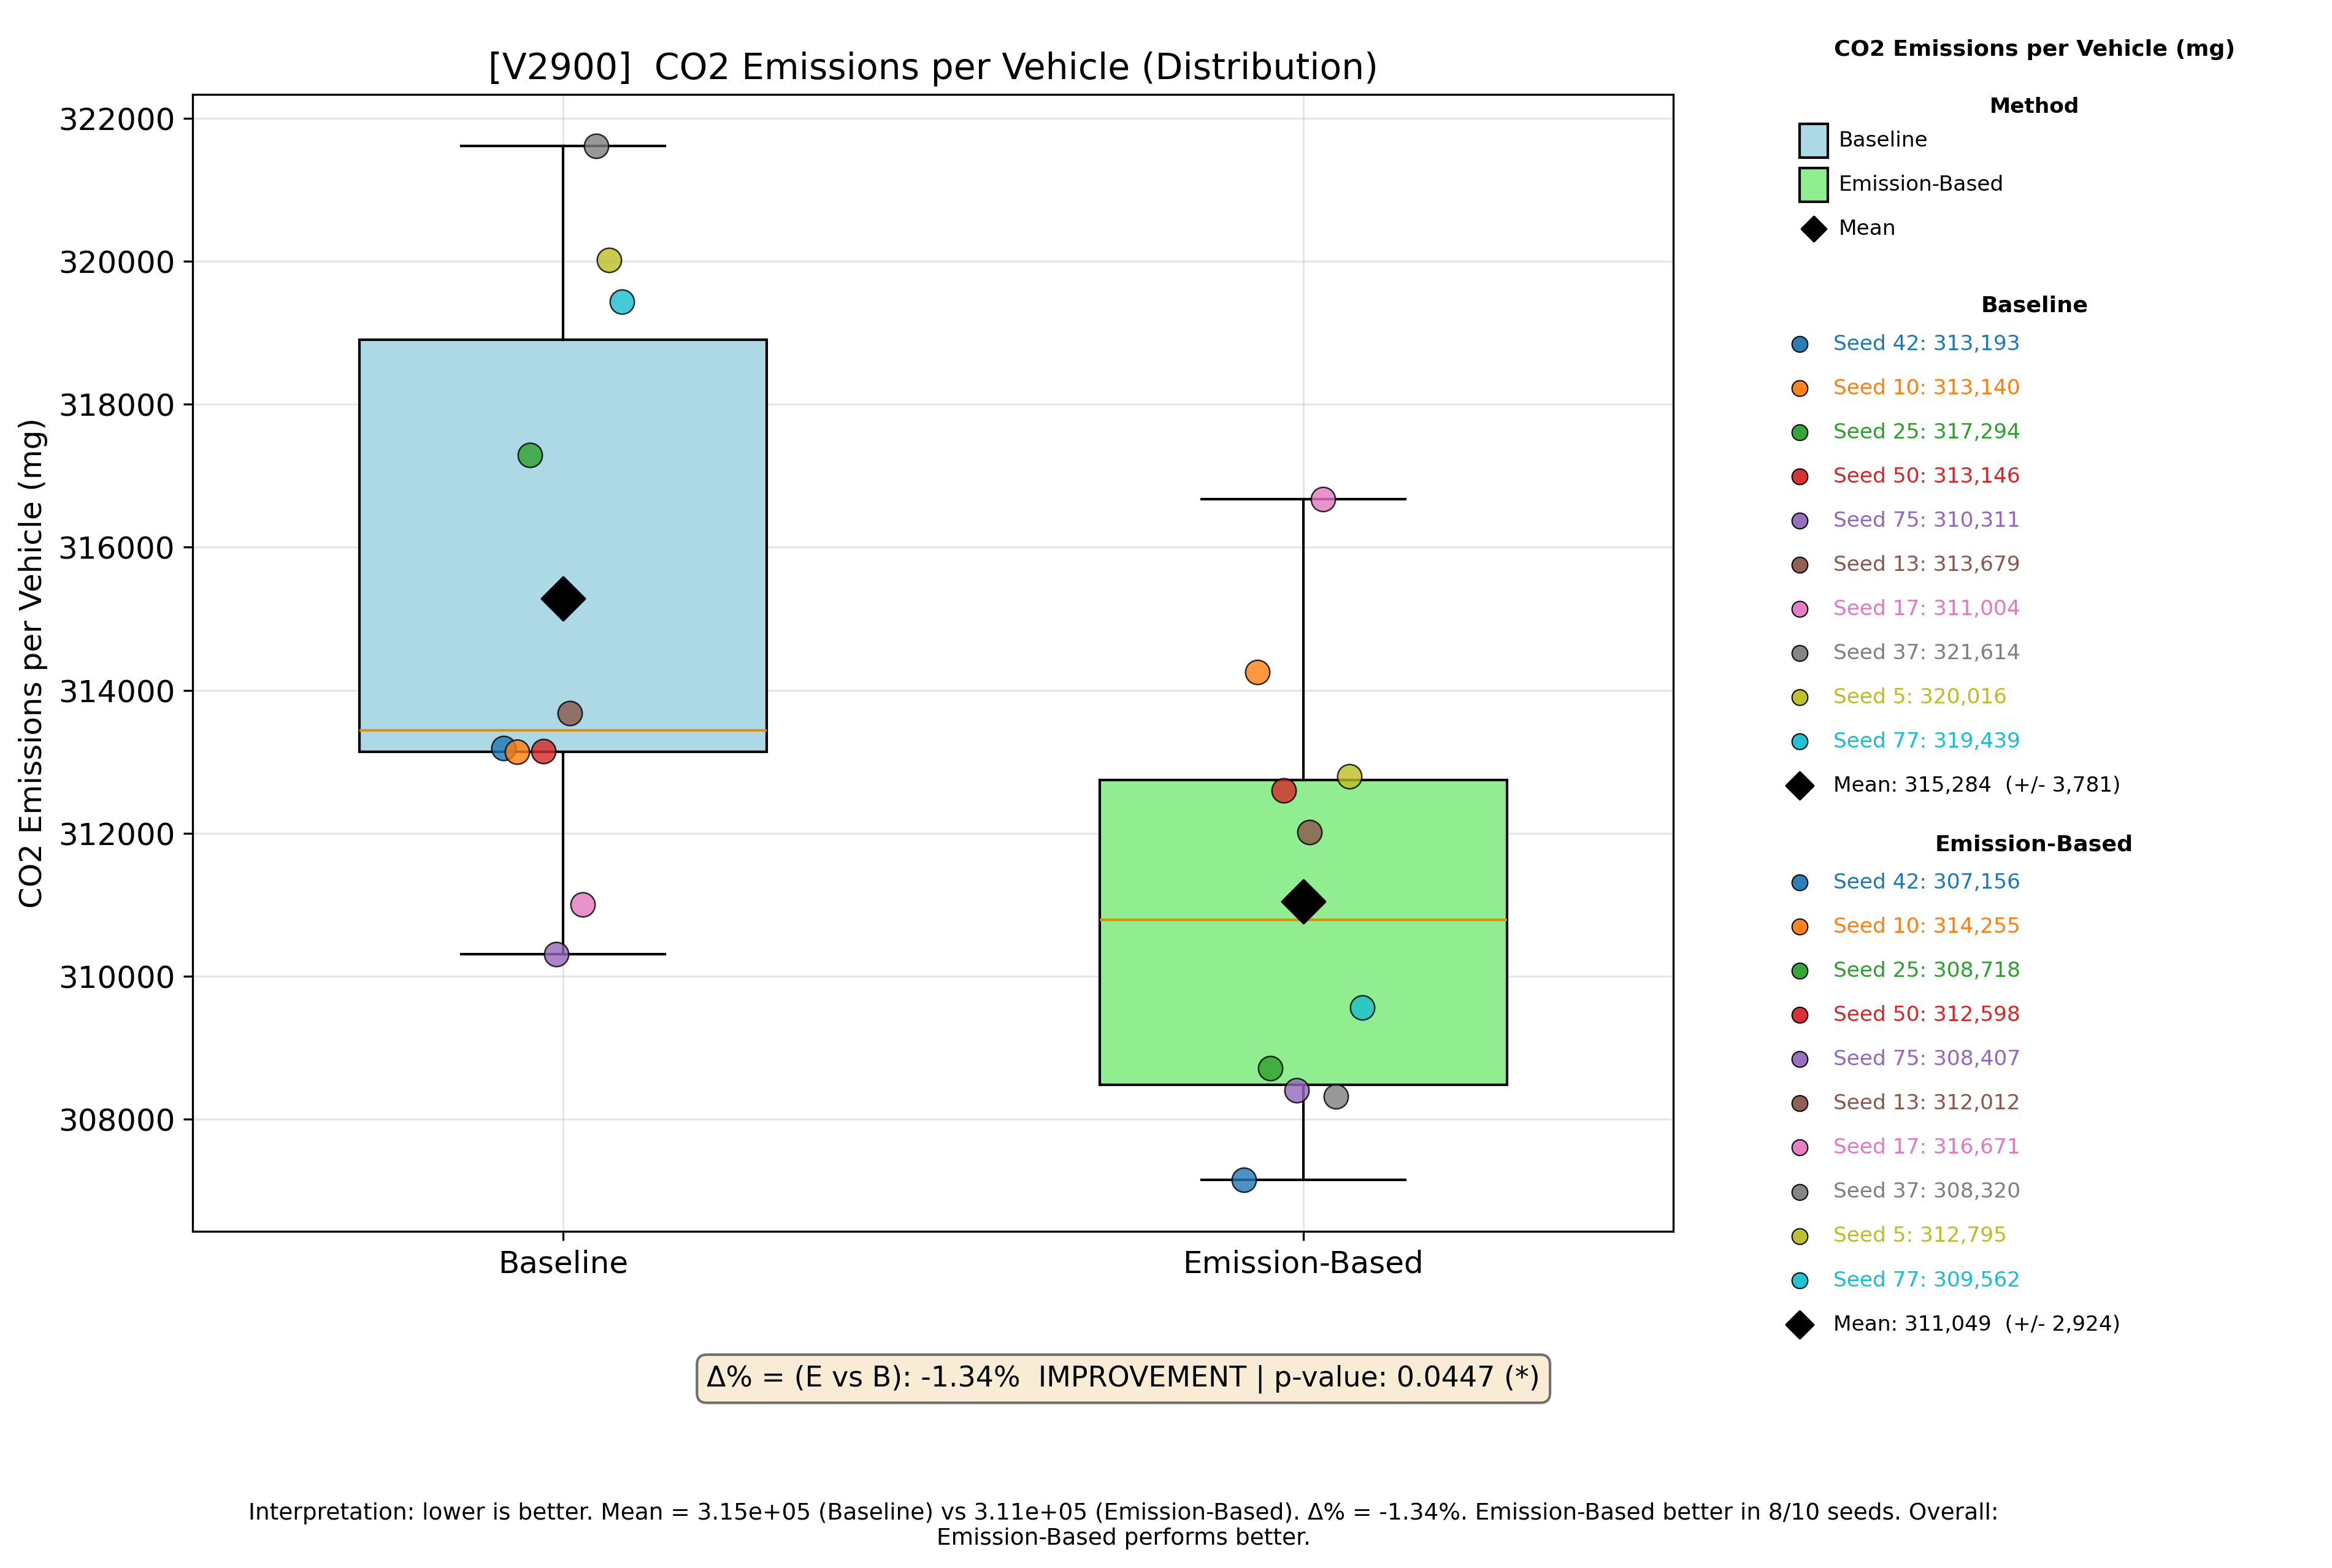
\includegraphics[width=0.85\textwidth]{visuals/V2900/single_boxplot_avg_co2_per_vehicle}
  \caption{V2900 (Near-saturation) CO$_2$/vehicle distribution. Statistically
    significant saving: $\Delta=-1.34\%$, paired $p=0.045$, 8/10 seeds.}
  \label{fig:v2900_box}
\end{figure}

\begin{figure}[H]
  \centering
  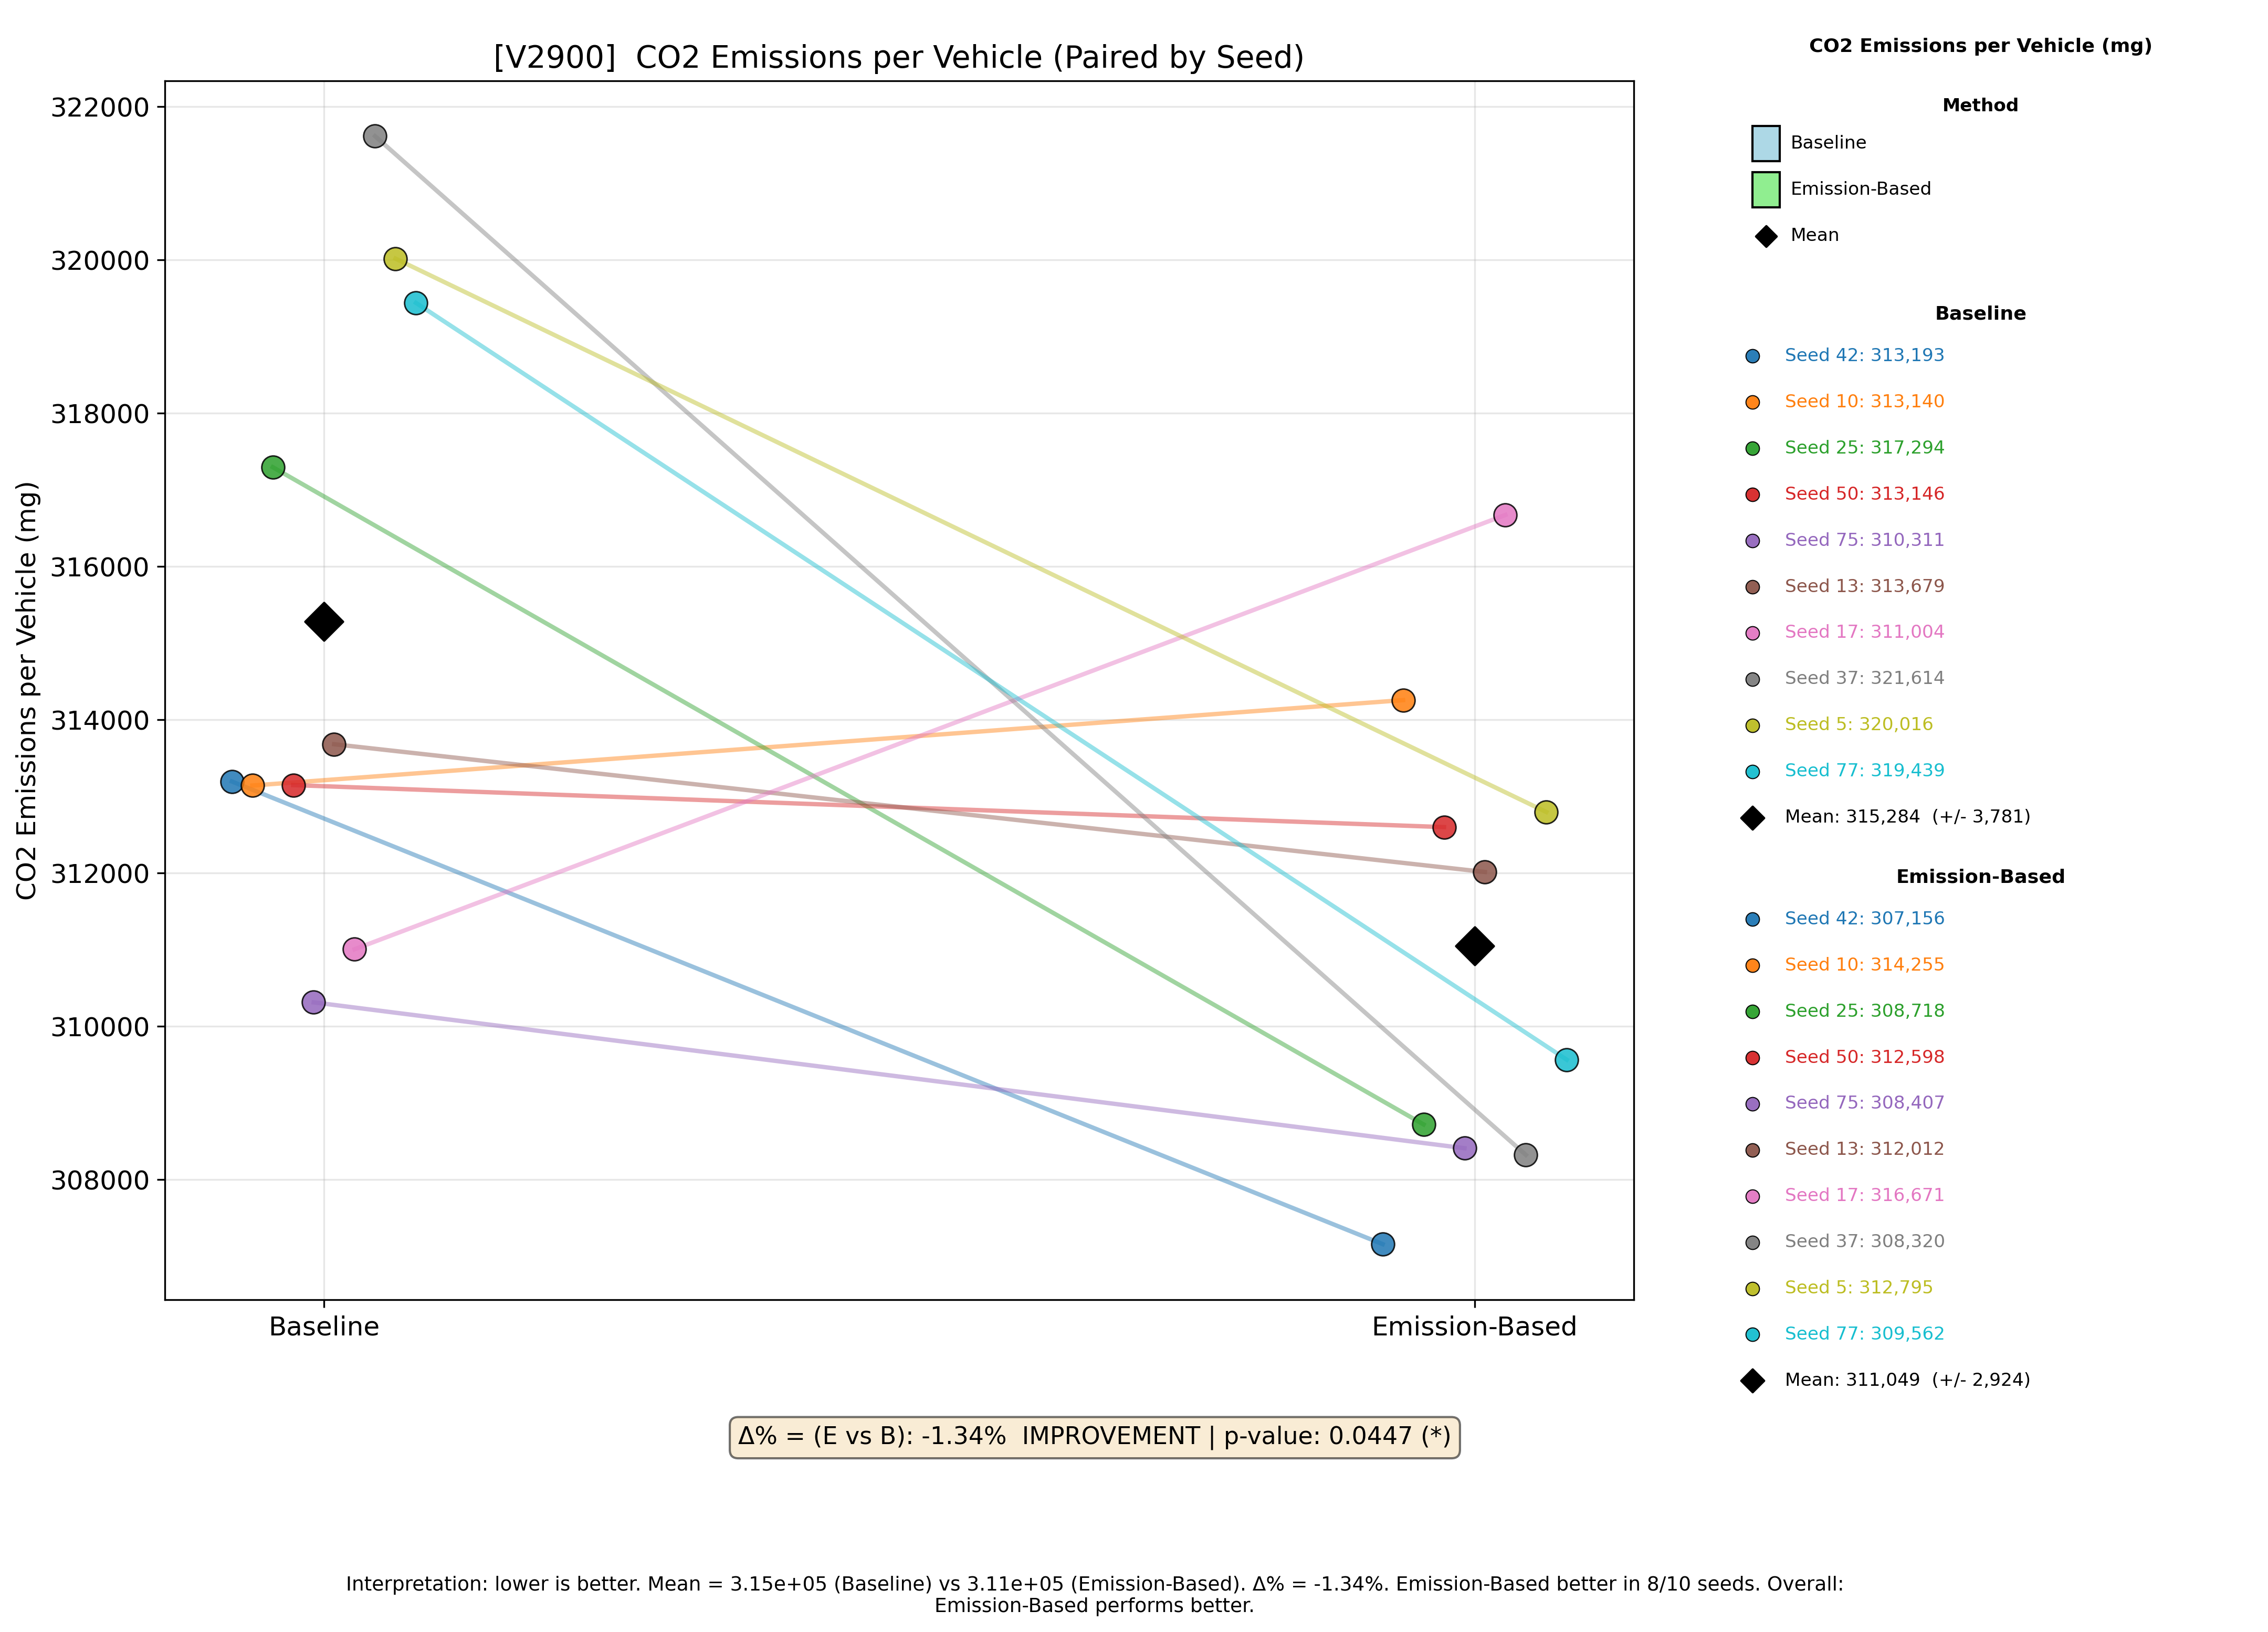
\includegraphics[width=0.85\textwidth]{visuals/V2900/single_paired_avg_co2_per_vehicle}
  \caption{V2900 paired-seed CO$_2$/vehicle comparison. Dominantly downward
    line slopes signal a controller-driven benefit consistent across seeds.}
  \label{fig:v2900_paired}
\end{figure}

\begin{figure}[H]
  \centering
  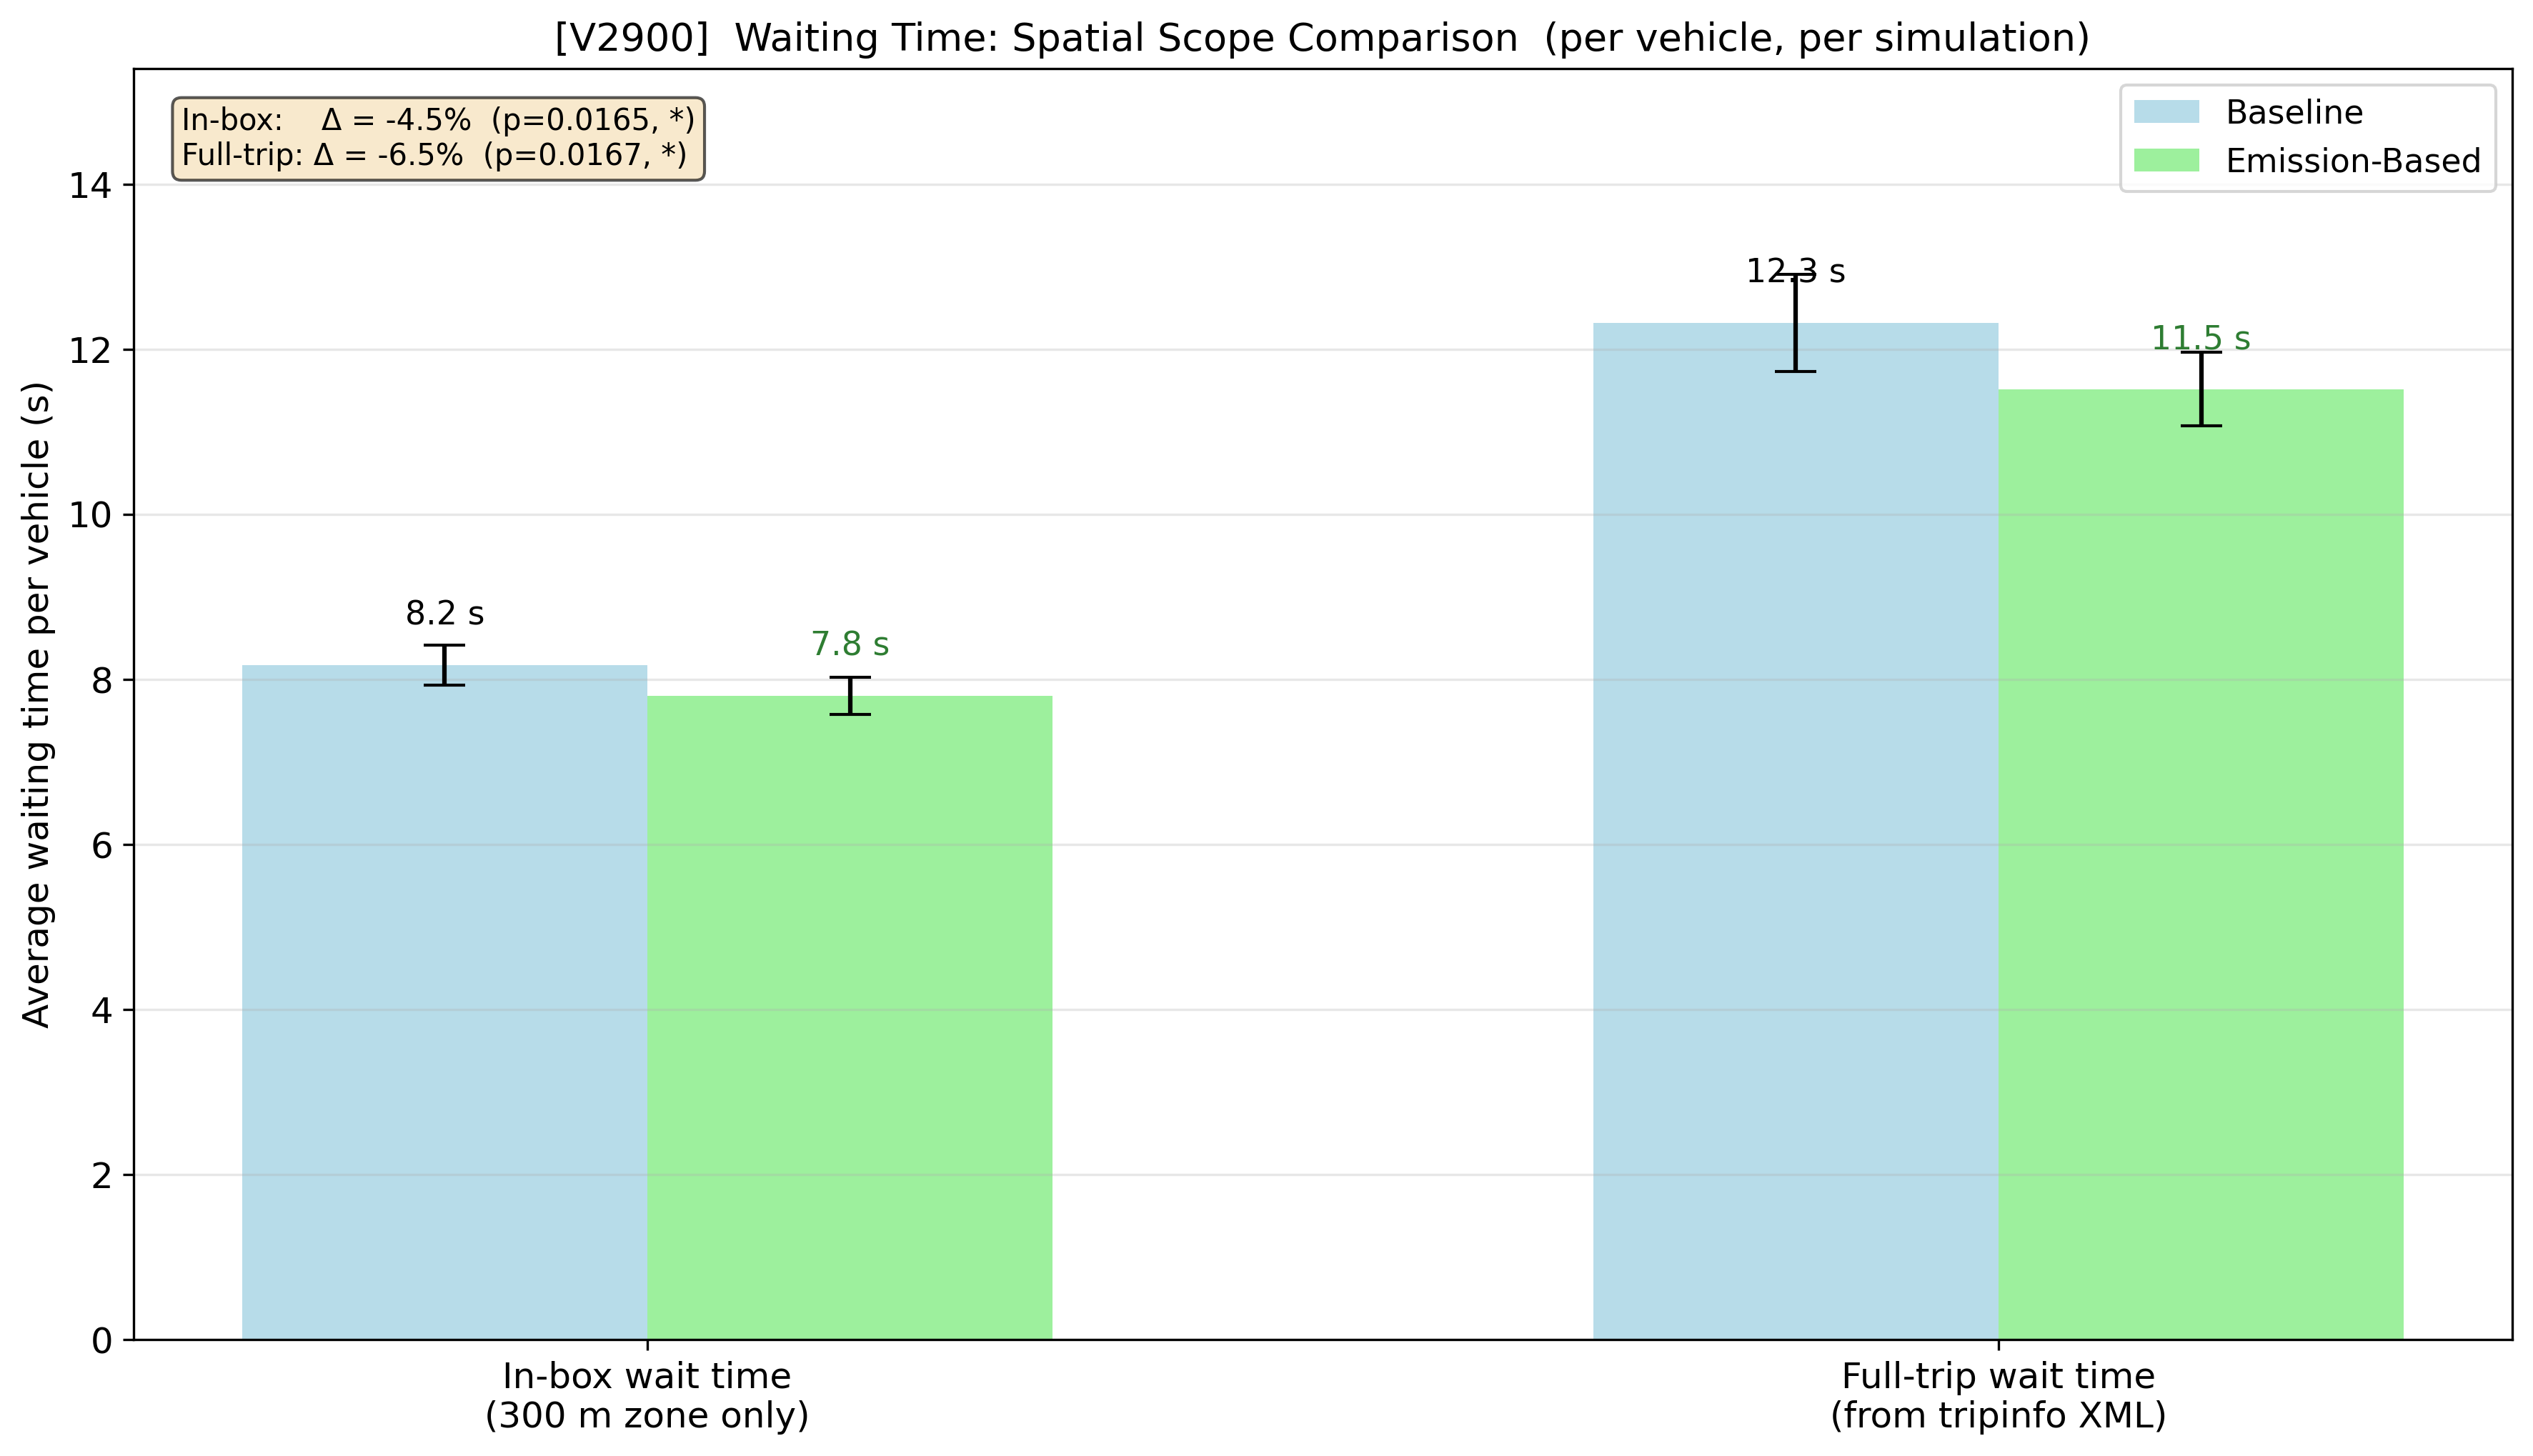
\includegraphics[width=0.85\textwidth]{visuals/V2900/dual_wait_time_comparison}
  \caption{V2900 wait time by seed. Both wait types fall under EBAC in every
    seed; the $\sim$4\,s in-box/full-trip gap reveals emerging approach-lane
    queuing.}
  \label{fig:v2900_dw}
\end{figure}

Near-saturation is EBAC's strongest regime. Savings of $+1.33\%$ at
$\text{thr}=50$ ($p=0.045$) and $+1.90\%$ at $\text{thr}=42$ ($p=0.007$)
are both statistically significant, and the large Cohen's $d$ values (1.19
and 1.67, respectively) indicate an effect that should replicate reliably.
Wait time falls by $7.9$--$8.7\%$ and phase-switch frequency decreases
relative to SAC.

\clearpage
\subsection{Breakdown Onset (V3300)}

\begin{figure}[H]
  \centering
  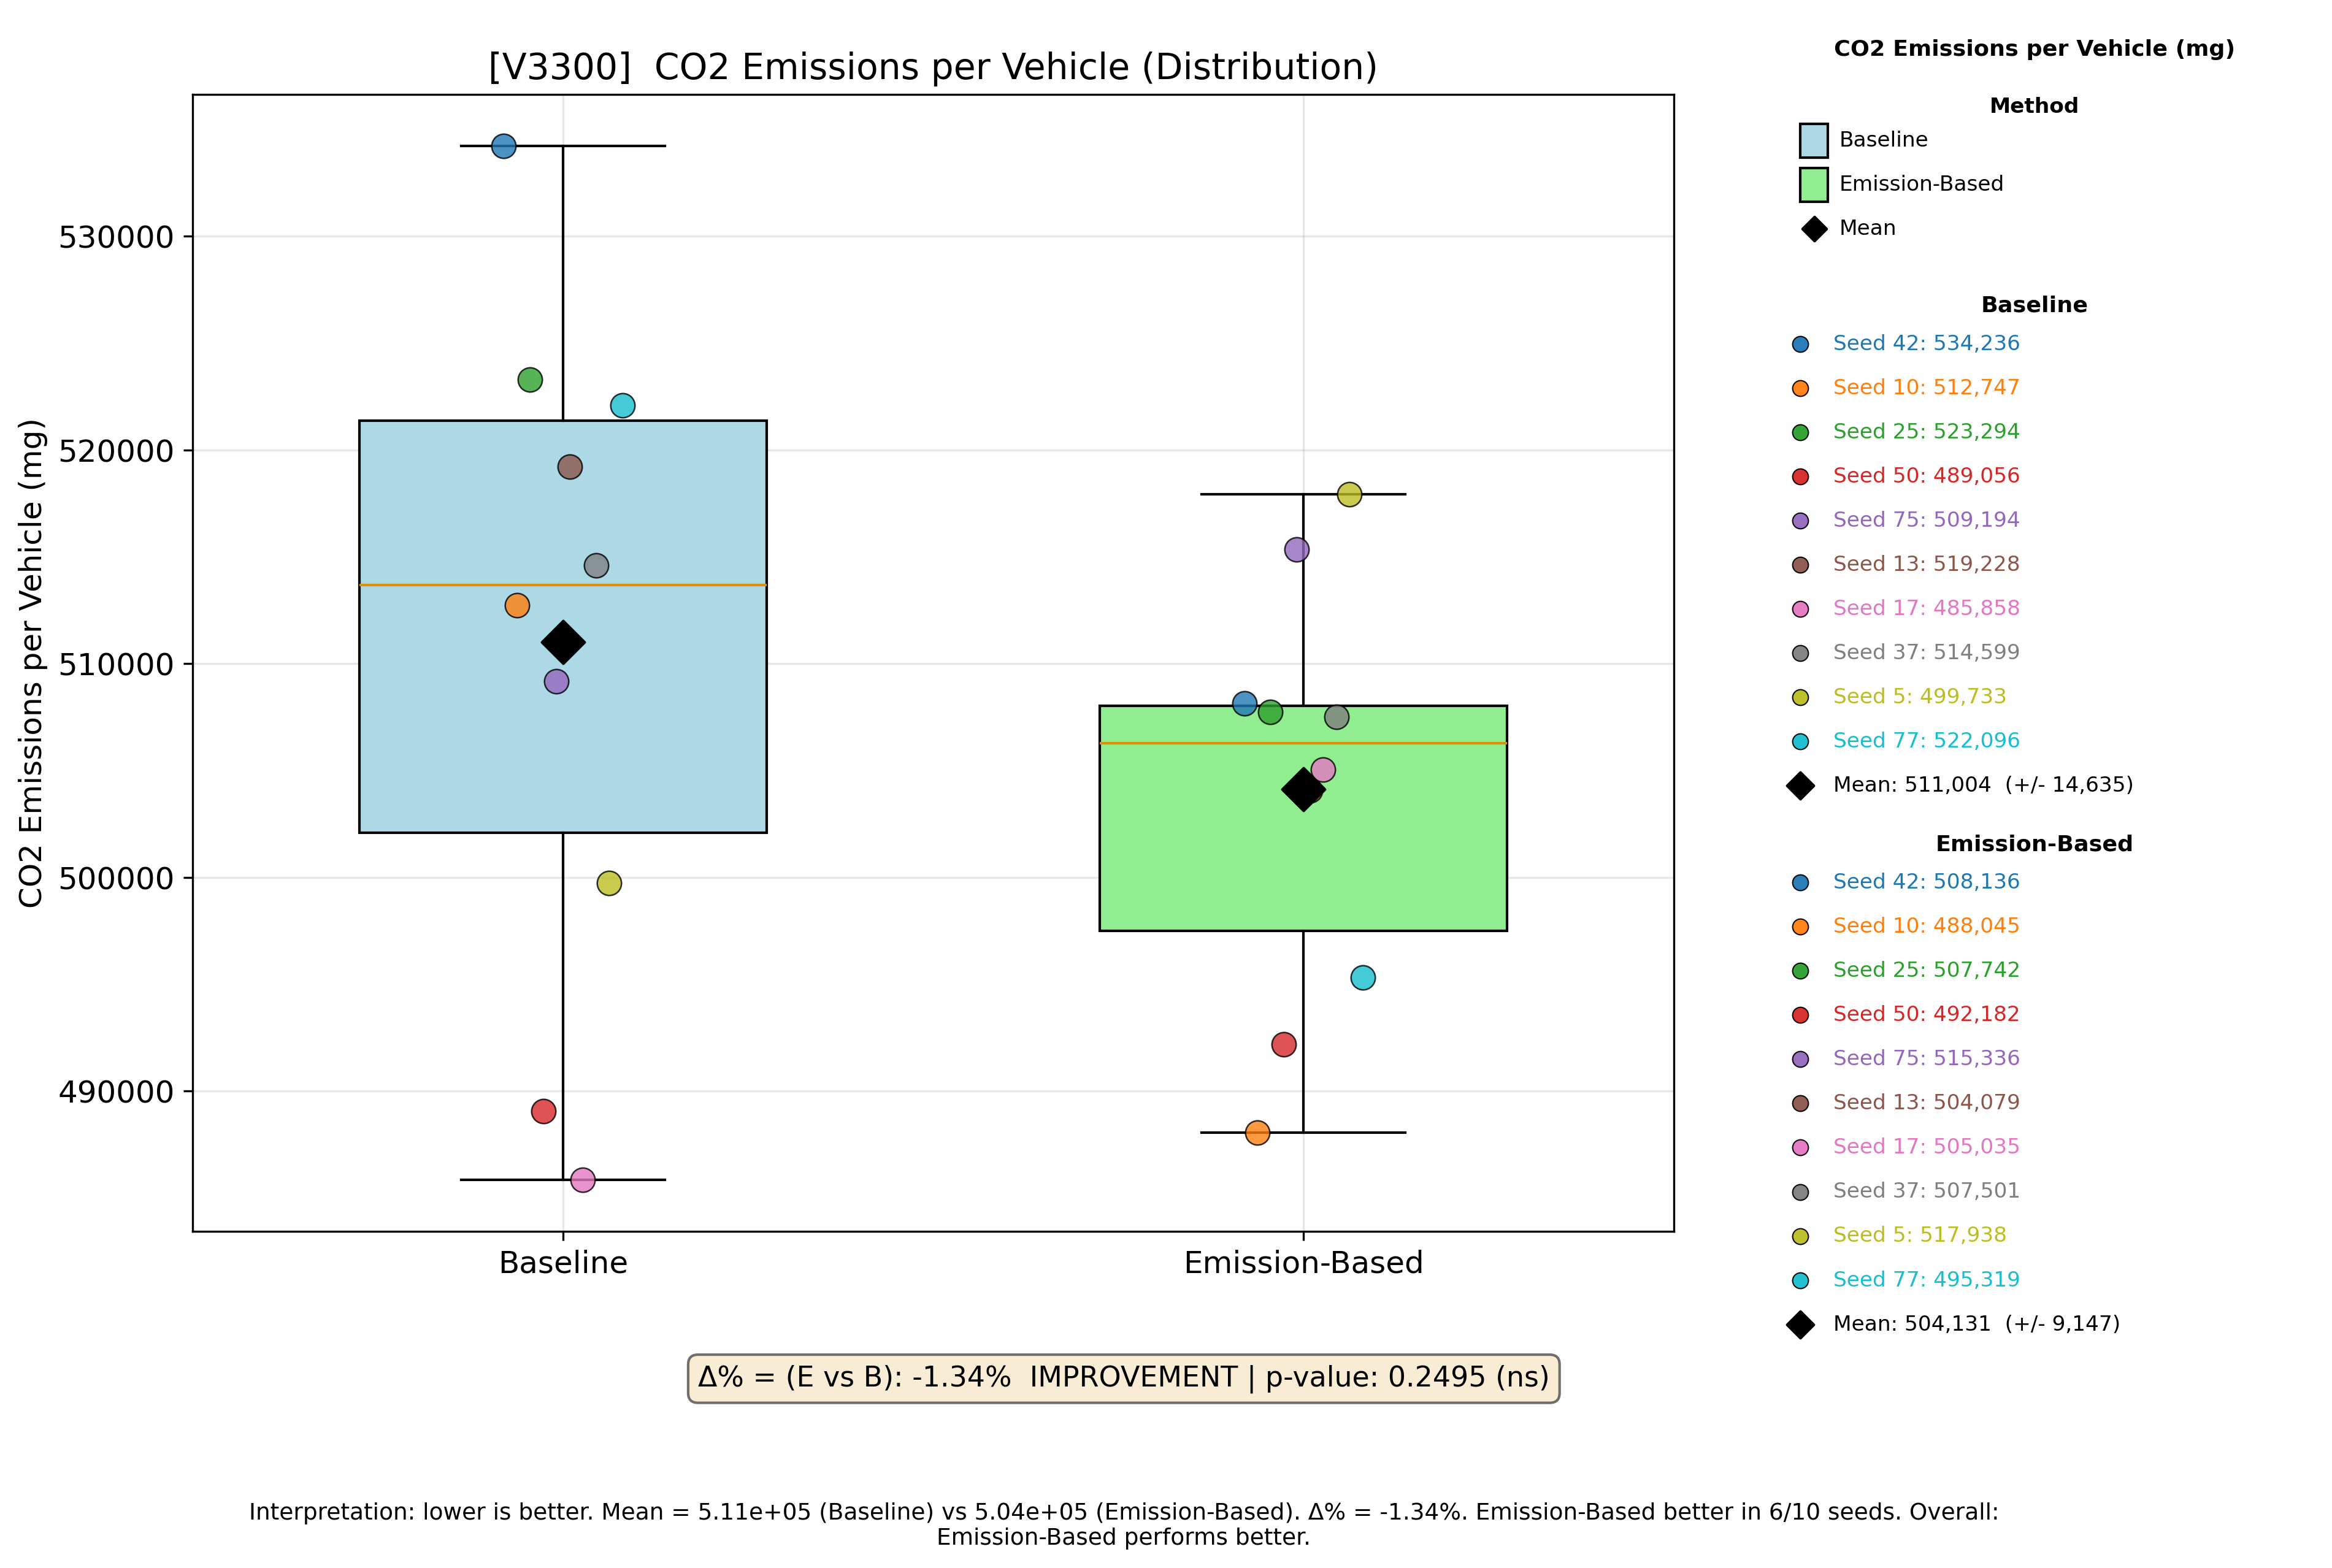
\includegraphics[width=0.85\textwidth]{visuals/V3300/single_boxplot_avg_co2_per_vehicle}
  \caption{V3300 (Breakdown onset) CO$_2$/vehicle distribution. Mean saving
    $\Delta=-1.34\%$, paired $p=0.25$, 6/10 seeds; larger between-seed variance
    than V2900 hides the effect under the null test.}
  \label{fig:v3300_box}
\end{figure}

\begin{figure}[H]
  \centering
  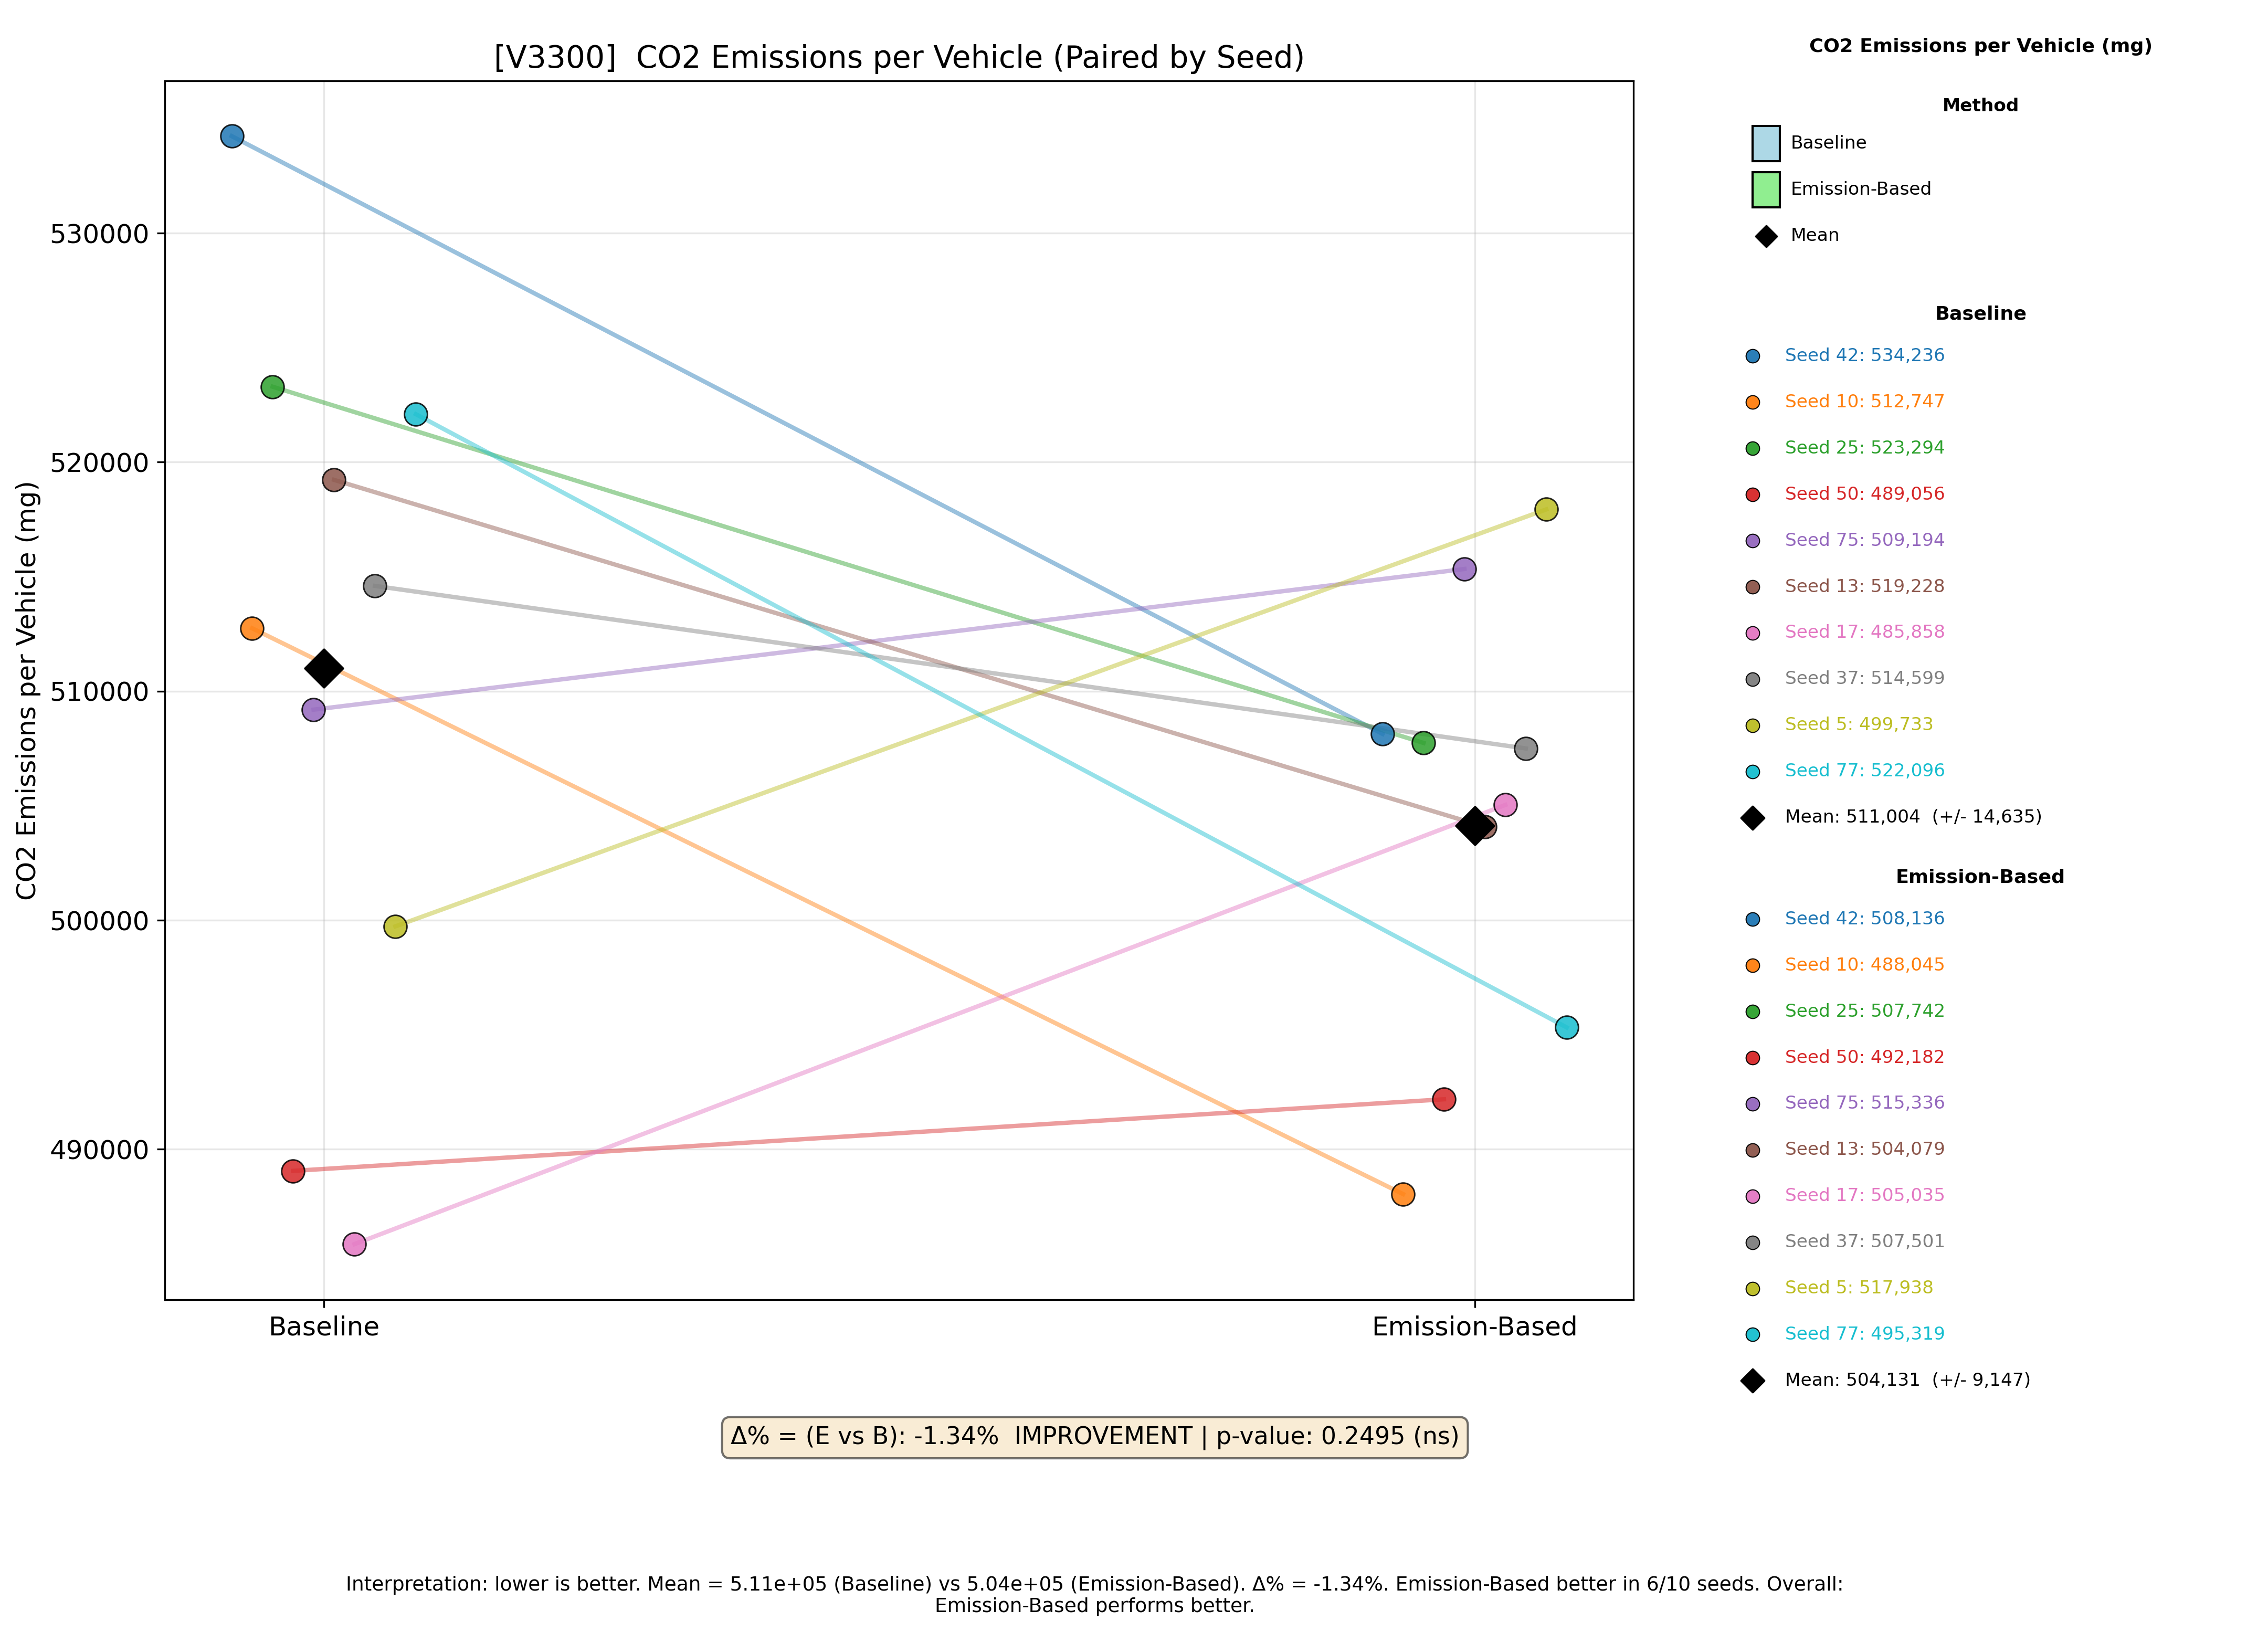
\includegraphics[width=0.85\textwidth]{visuals/V3300/single_paired_avg_co2_per_vehicle}
  \caption{V3300 paired-seed CO$_2$/vehicle comparison. Predominantly downward
    slopes with two inversions; variance-limited rather than effect-limited.}
  \label{fig:v3300_paired}
\end{figure}

\begin{figure}[H]
  \centering
  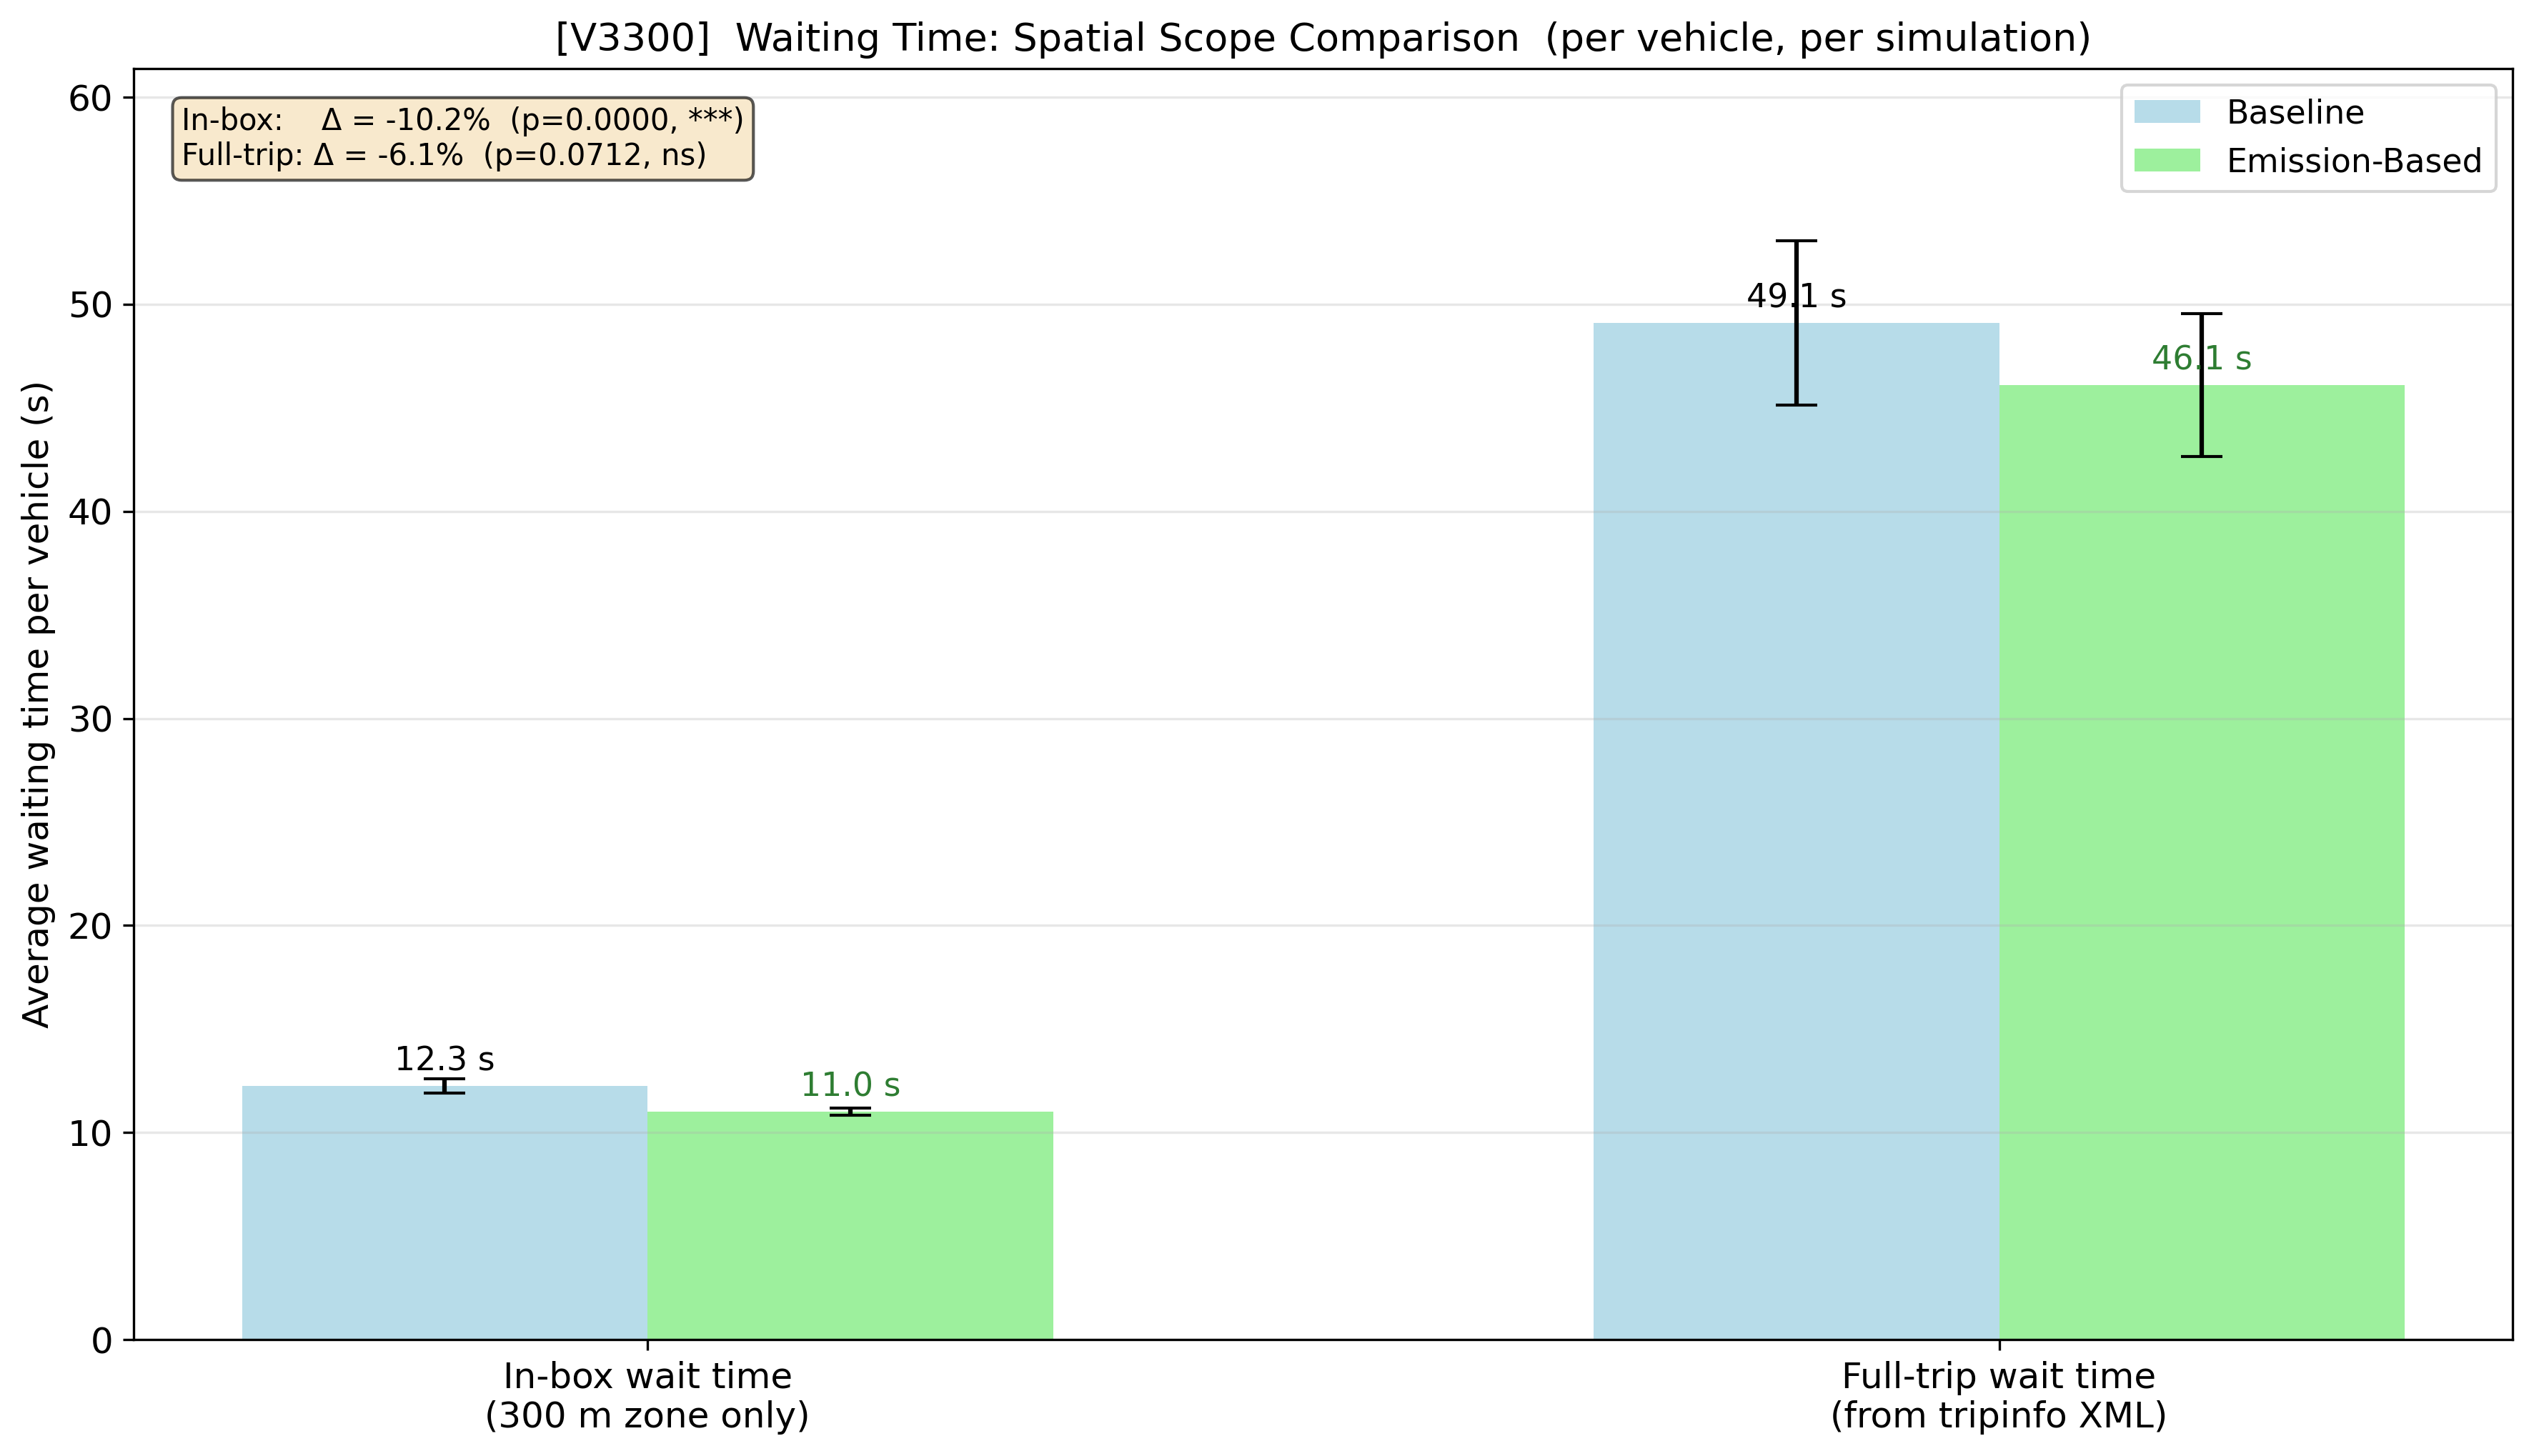
\includegraphics[width=0.85\textwidth]{visuals/V3300/dual_wait_time_comparison}
  \caption{V3300 wait time by seed. The $\sim$35--40\,s in-box/full-trip gap is
    approach-lane wait; EBAC lowers in-box wait in every seed.}
  \label{fig:v3300_dw}
\end{figure}

Breakdown onset delivers the highest post-hoc saving ($+3.01\%$ at
$\text{thr}=135$), though the seed-to-seed variance is inflated by
queue-spillback dynamics. We interpret the non-significance at
$\text{thr}=50$ ($+1.27\%$, $p=0.249$, $d=0.53$) as a variance problem
rather than an absence of effect---the underlying direction is consistent,
but stochastic spillback events shift the magnitude substantially from seed
to seed. Wait time falls by $13.6\%$ at optimum, the second-largest
reduction across all four regimes.

\clearpage
\subsection{Gridlock (V5000)}

\begin{figure}[H]
  \centering
  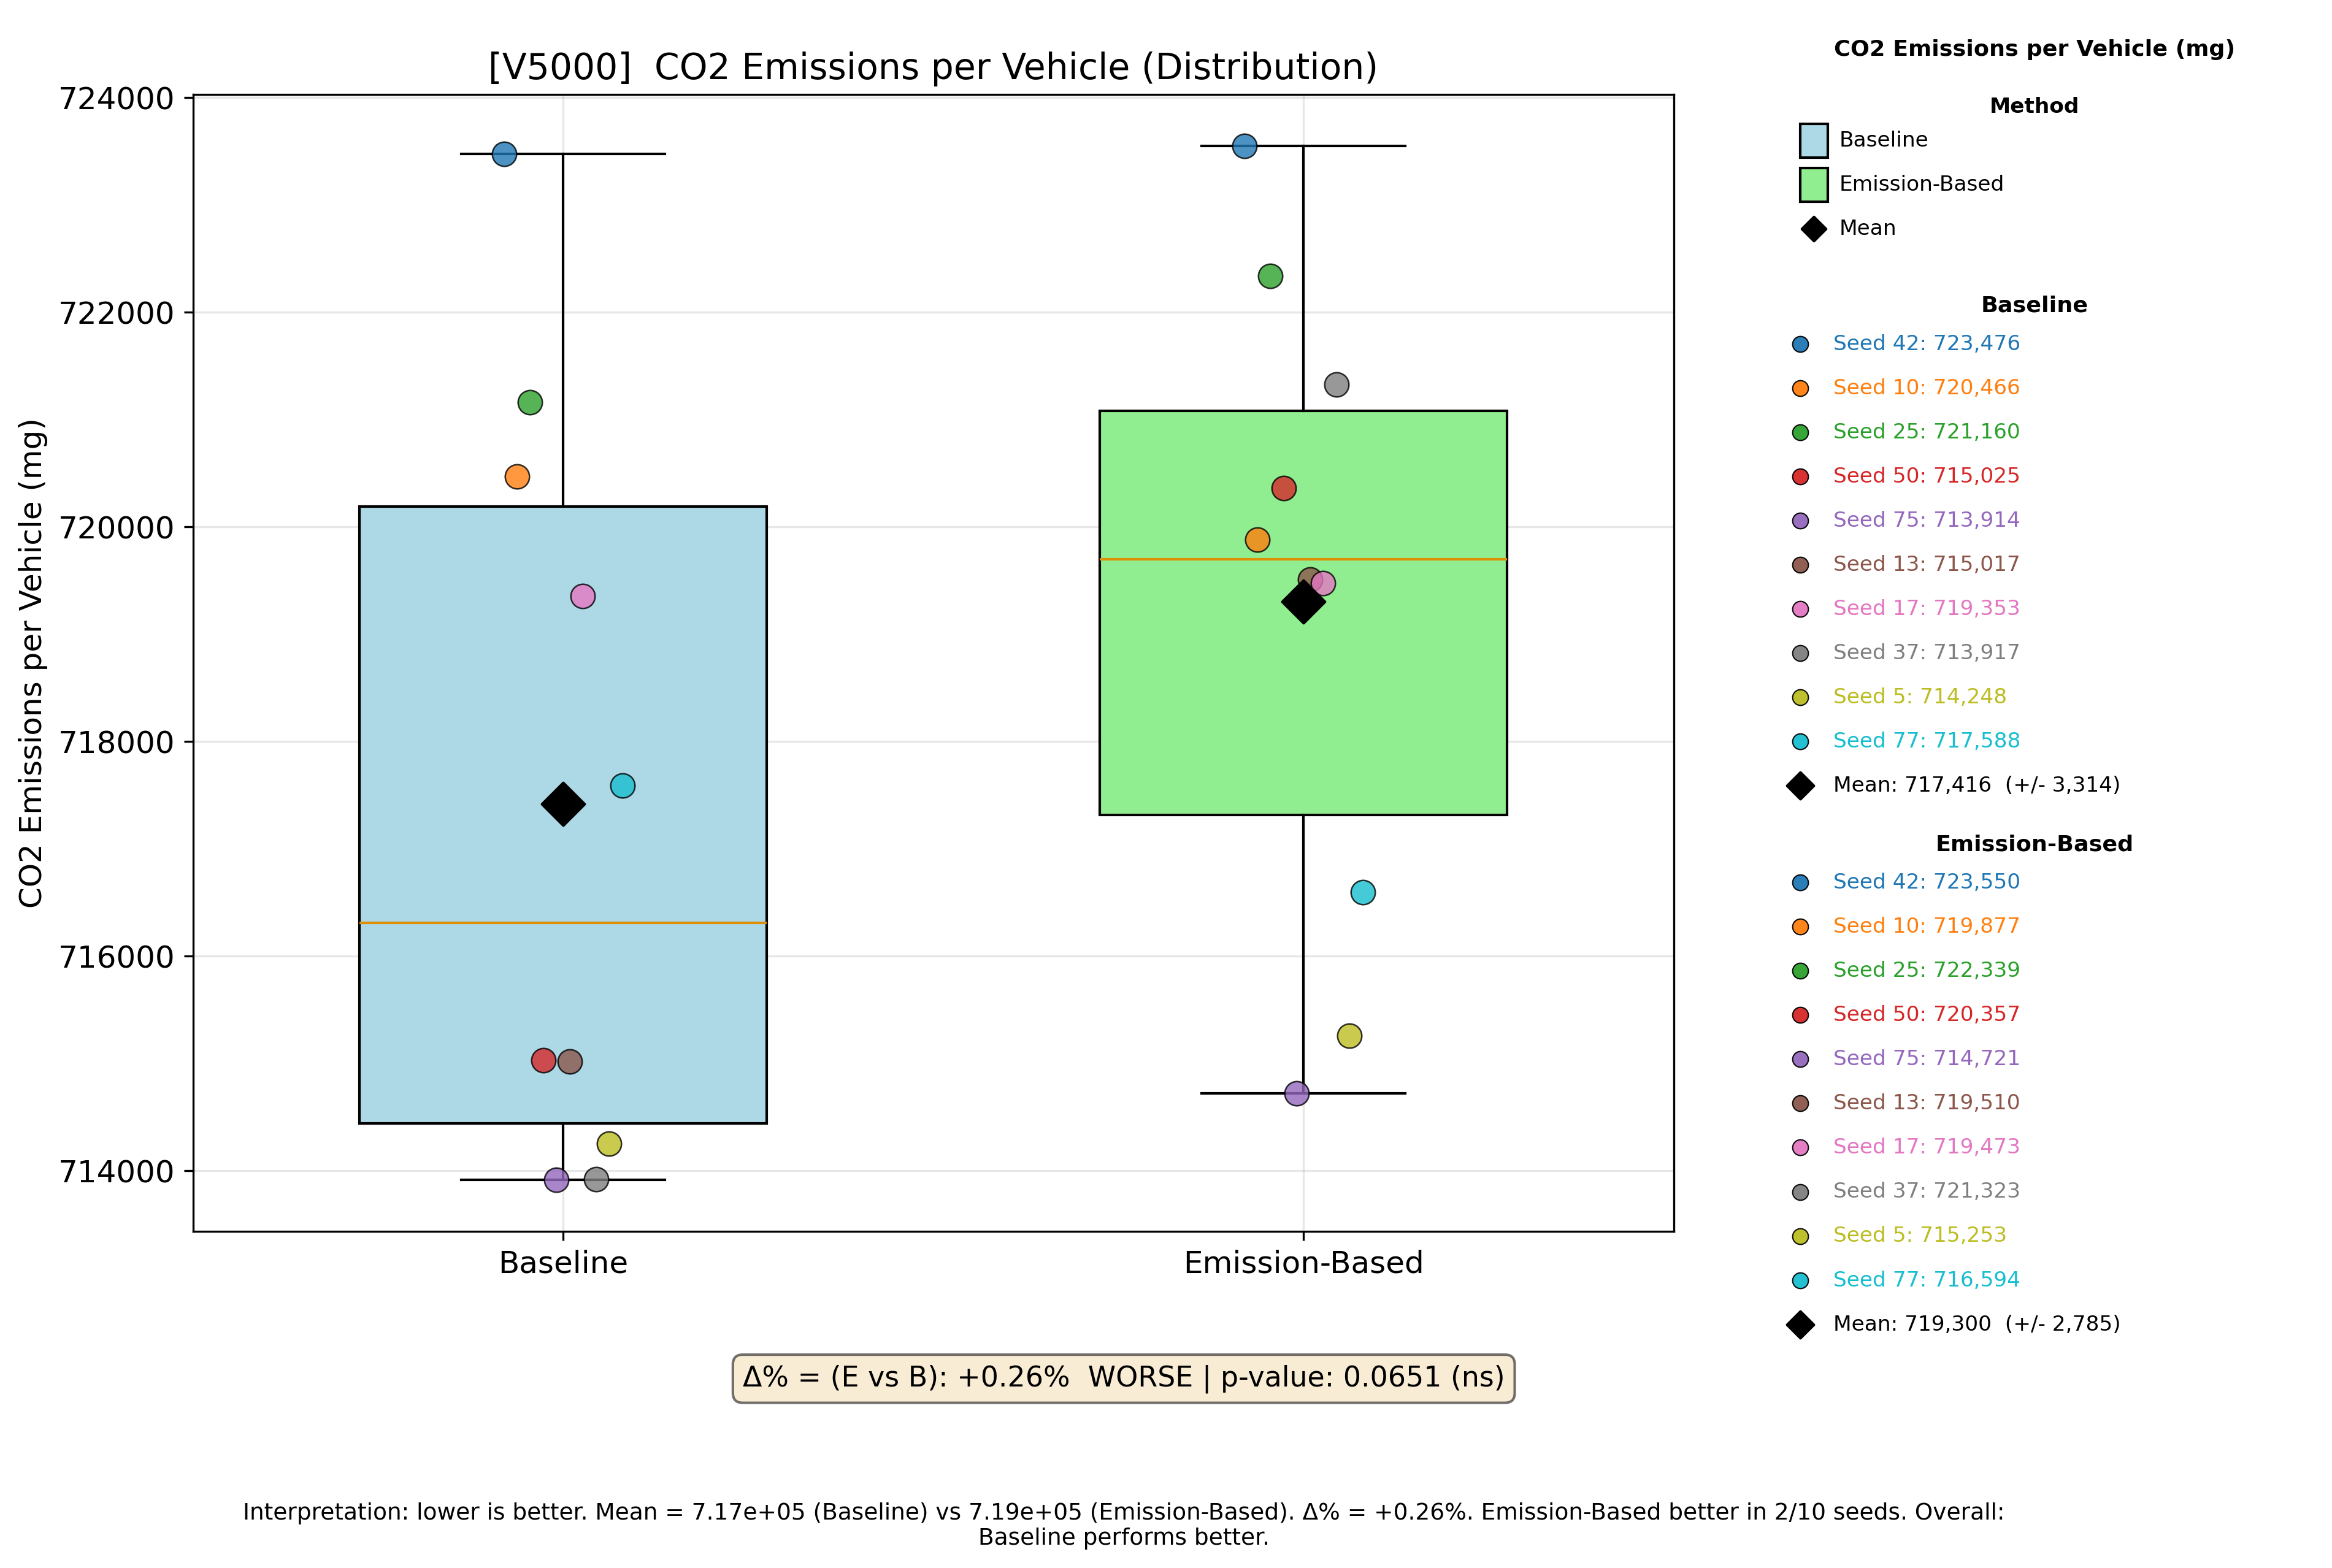
\includegraphics[width=0.85\textwidth]{visuals/V5000/single_boxplot_avg_co2_per_vehicle}
  \caption{V5000 (Gridlock) CO$_2$/vehicle distribution. Cross-over regime:
    $\Delta=+0.26\%$ (WORSE at $\text{thr}=50$), 2/10 seeds; both approaches
    saturated so the asymmetry EBAC exploits vanishes.}
  \label{fig:v5000_box}
\end{figure}

\begin{figure}[H]
  \centering
  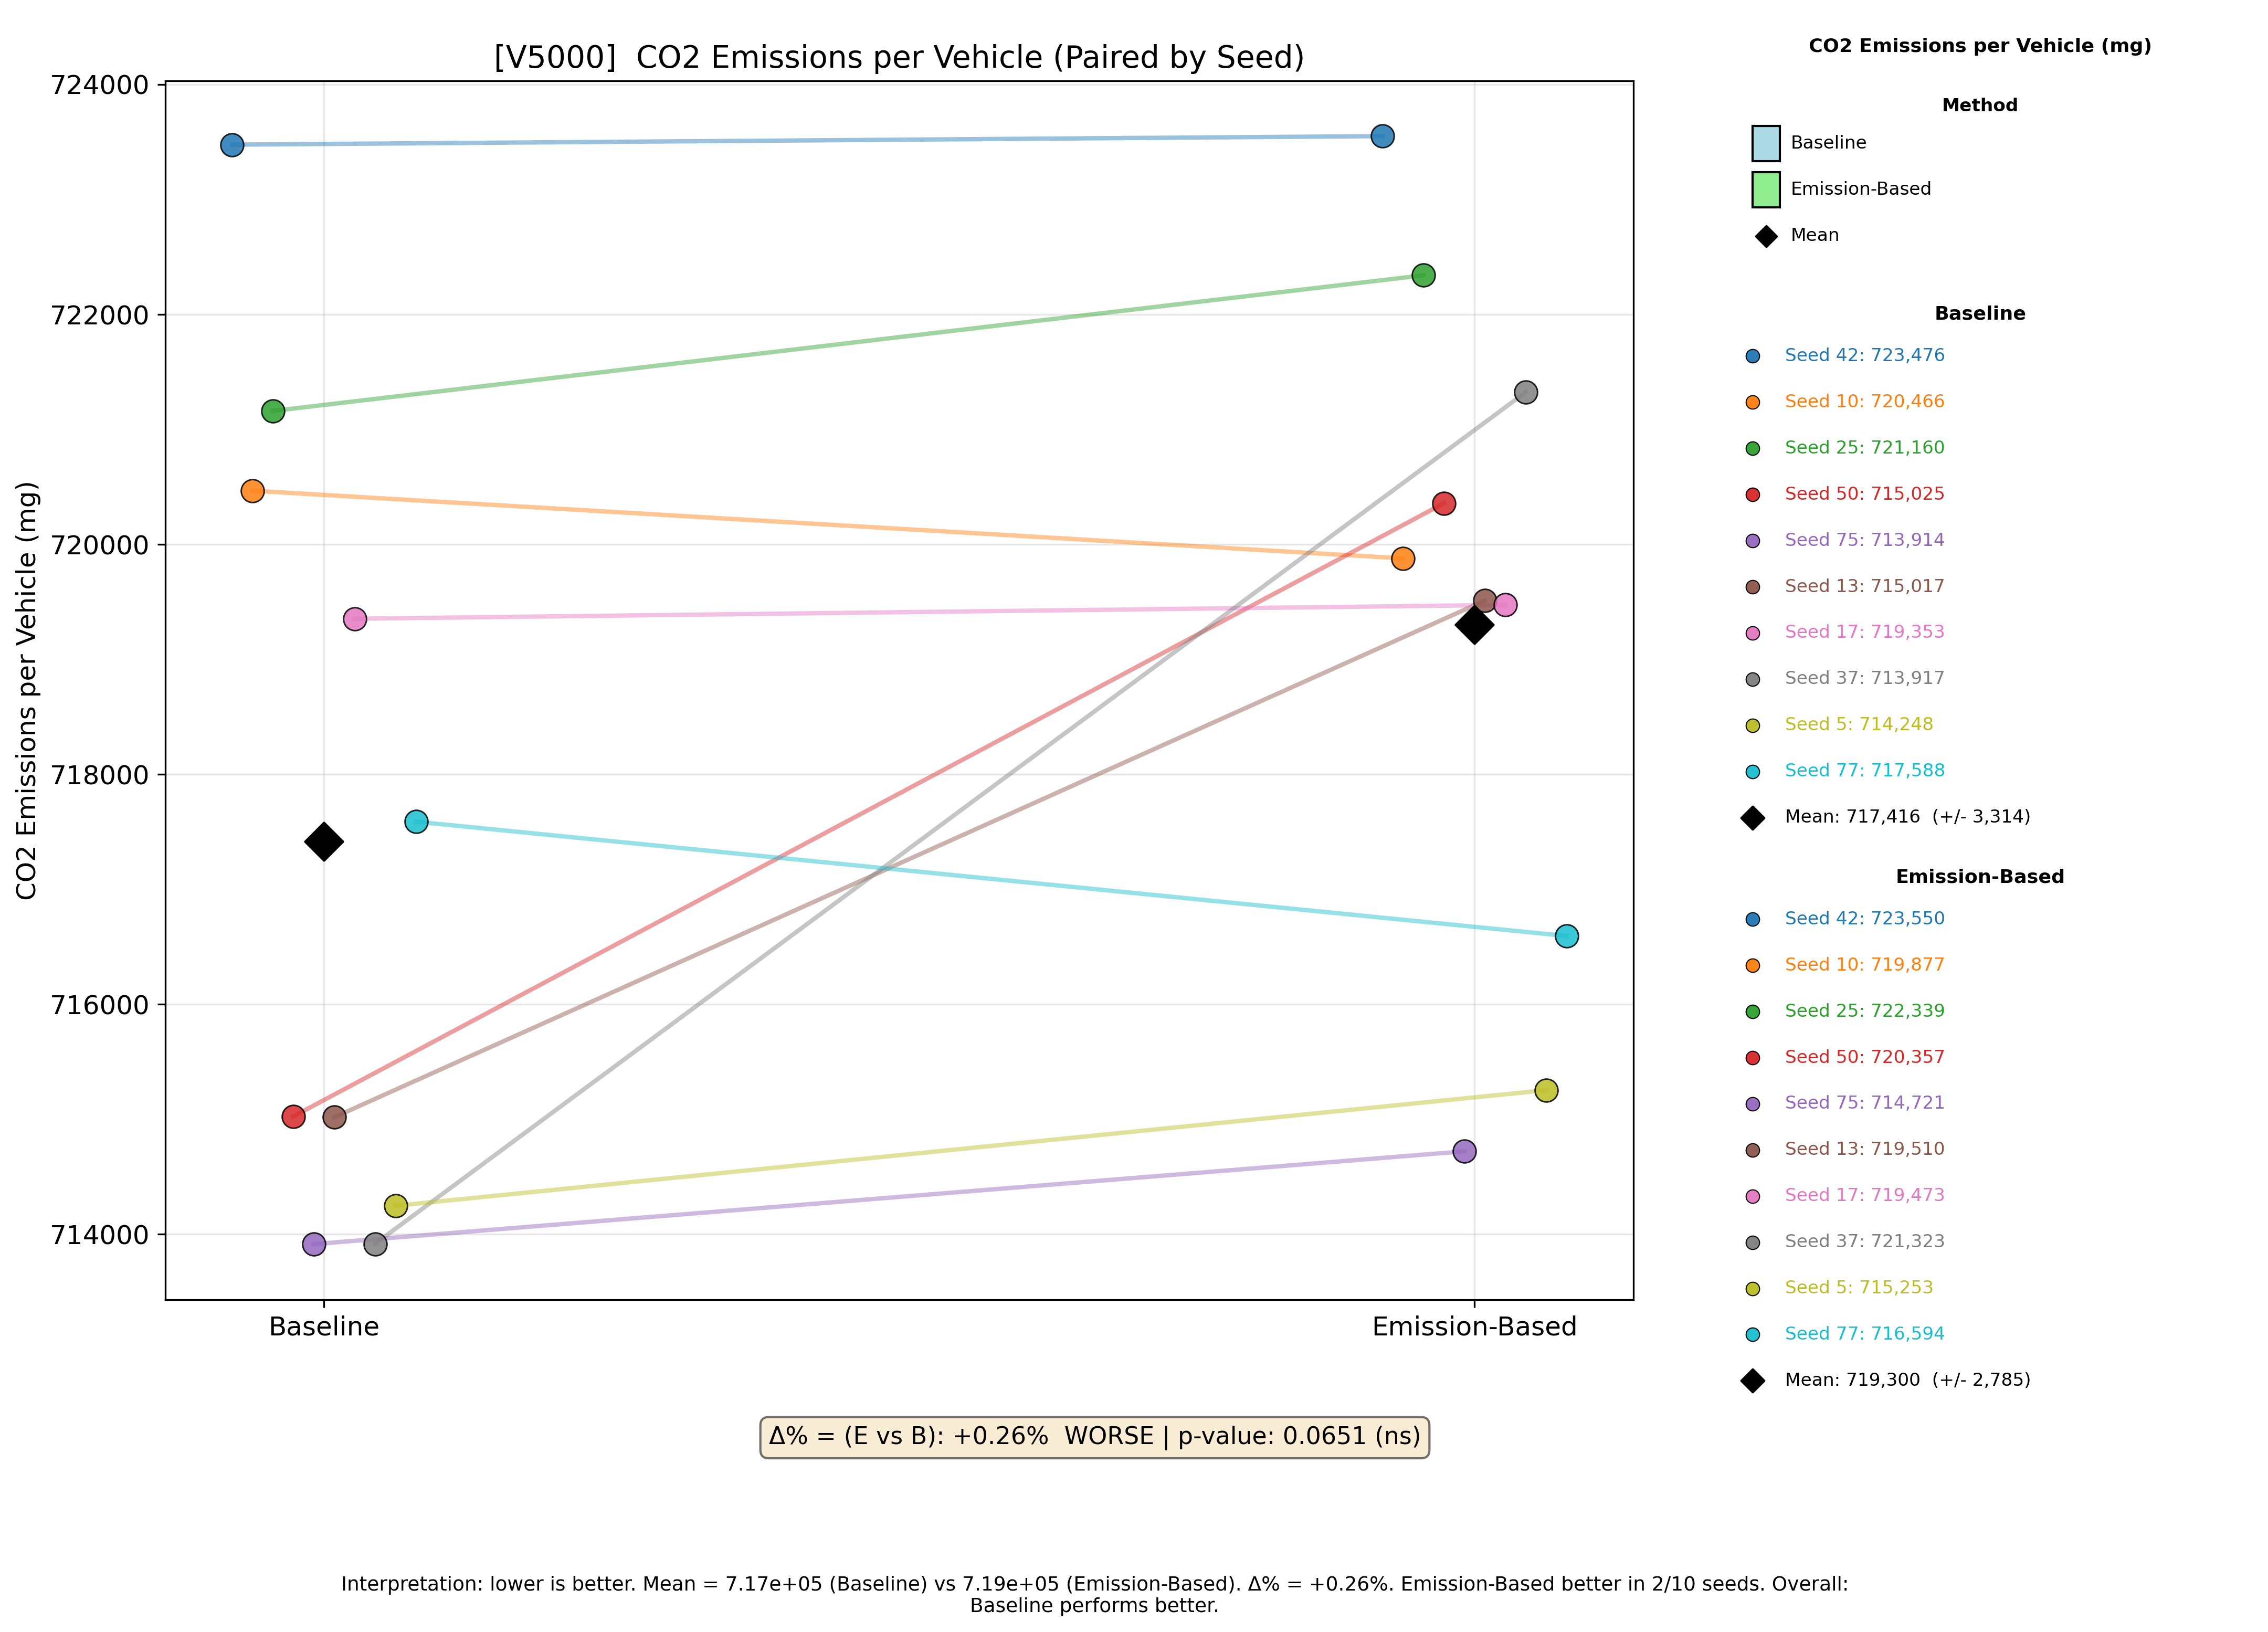
\includegraphics[width=0.85\textwidth]{visuals/V5000/single_paired_avg_co2_per_vehicle}
  \caption{V5000 paired-seed CO$_2$/vehicle comparison. Predominantly upward
    slopes---the visual inverse of V2900.}
  \label{fig:v5000_paired}
\end{figure}

\begin{figure}[H]
  \centering
  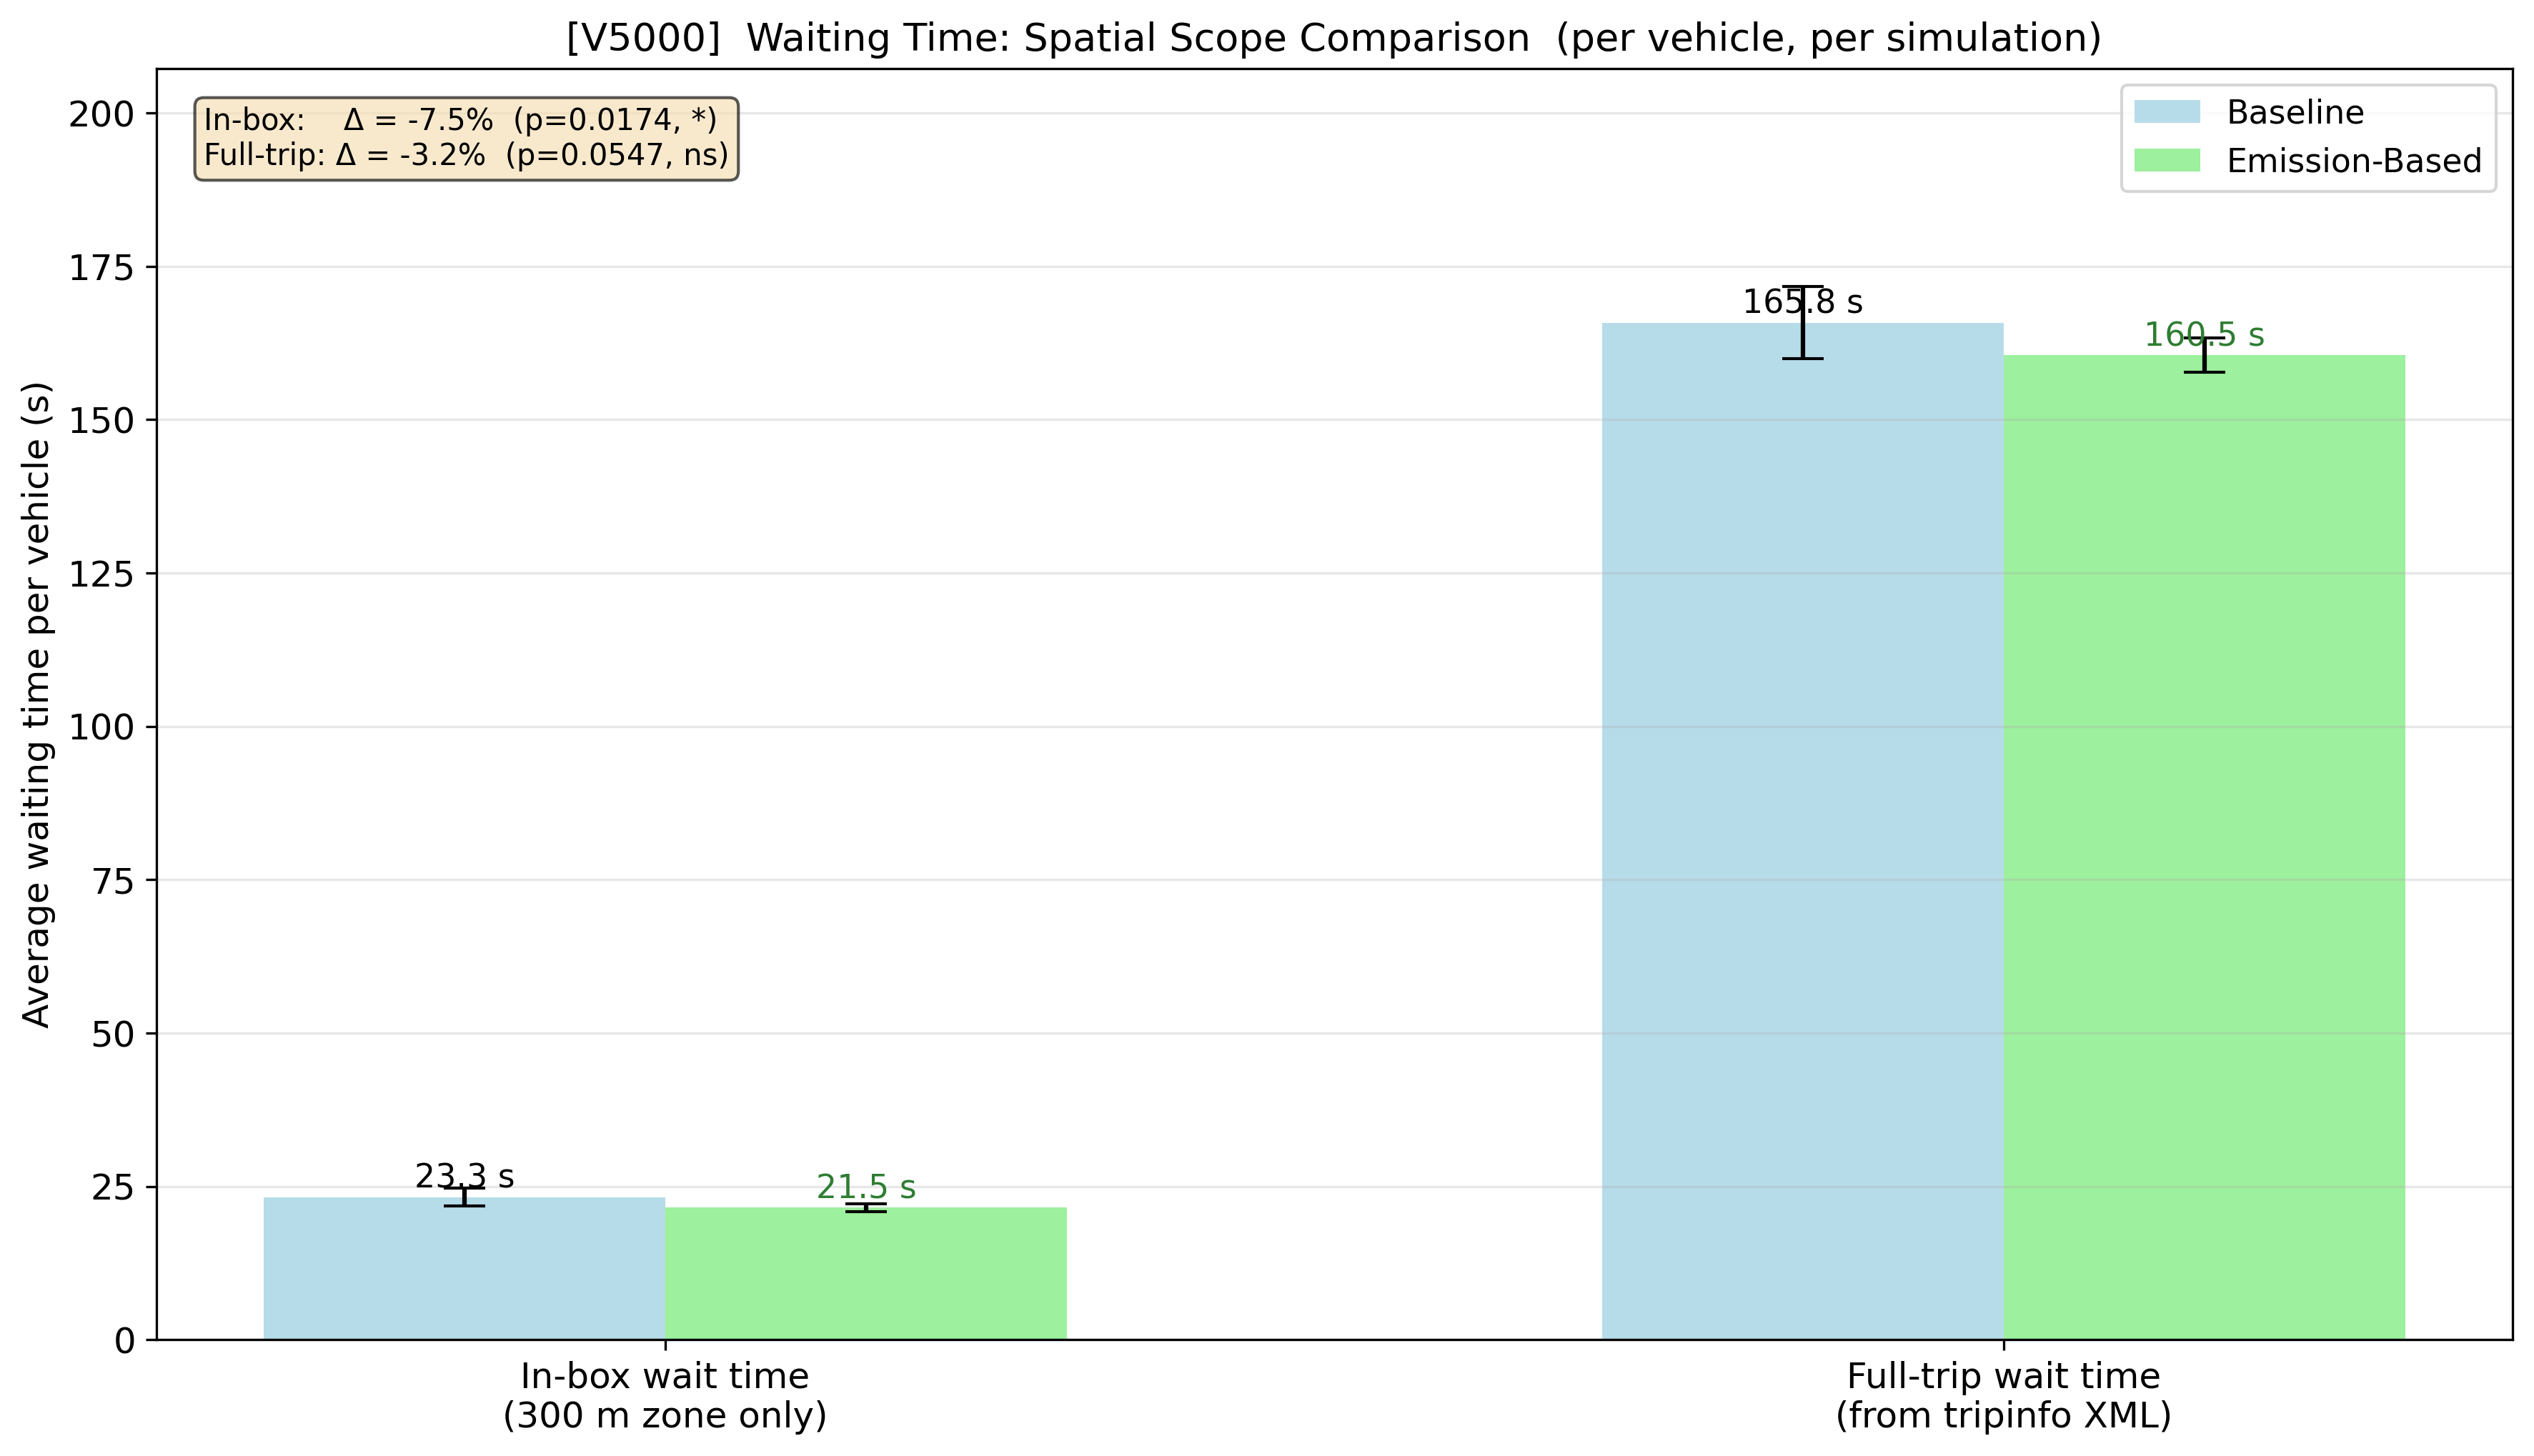
\includegraphics[width=0.85\textwidth]{visuals/V5000/dual_wait_time_comparison}
  \caption{V5000 wait time by seed. Full-trip wait ($\sim$155--175\,s)
    dwarfs in-box wait ($\sim$21--26\,s); the $\sim$140\,s gap is
    approach-lane queueing. EBAC still reduces both wait types by 1--15\,s.}
  \label{fig:v5000_dw}
\end{figure}

At Gridlock, the emission asymmetry EBAC depends on largely disappears.
The optimum ($\text{thr}=138$) still yields wait-time reductions of
$15.0\%$---EBAC is not entirely without effect here---but
CO\textsubscript{2} savings collapse to $+0.20\%$ ($p=0.37$, $d=0.43$).
This regime marks the practical deployment boundary of the strategy.

\clearpage
\subsection{Regime Matrix Summary}

Fig.~\ref{fig:regime_matrix} consolidates all twelve per-regime panels into
a single publication-grade matrix. The row structure (CO\textsubscript{2}
boxplot, paired CO\textsubscript{2}, dual wait time) makes the four-regime
arc visible at a glance: EBAC transitions from irrelevant (Free-flow)
$\rightarrow$ beneficial and statistically significant (Near-saturation)
$\rightarrow$ variance-limited but directionally consistent (Breakdown)
$\rightarrow$ inverted on CO\textsubscript{2} but still helpful on wait
(Gridlock).

\begin{figure}[H]
  \centering
  \includegraphics[width=0.98\linewidth]%
    {visuals/cross_volume/regime_matrix}
  \caption{Per-regime results matrix (B = baseline, E = emission-aware; 10
    seeds/volume). Rows: CO$_2$/veh boxplot, CO$_2$/veh paired seed, wait
    time per seed. Columns: V1500, V2900, V3300, V5000. Per-column banners
    show mean $\Delta$, paired $p$, and per-seed win count.}
  \label{fig:regime_matrix}
\end{figure}

%% ============================================================
\FloatBarrier
\section{Cross-Volume Context}
\label{sec:crossvol}

The per-regime results are embedded in a full sweep of 71 demand volumes
(500--7\,500\,veh/hr) with 10 seeds each. Fig.~\ref{fig:crossvol} plots six
operational metrics across this range; Fig.~\ref{fig:narrative} isolates the
wait/trip/switch/CO$_2$ narrative.

\begin{figure}[H]
  \centering
  \includegraphics[width=\linewidth]%
    {visuals/cross_volume/cross_volume_comparison}
  \caption{Cross-volume comparison of six metrics: baseline (blue solid) vs.
    emission-aware (green dashed); mean $\pm$1\,SD across seeds. The two
    controllers are visually indistinguishable at this aggregation scale except
    for in-box wait (panel~b) once demand exceeds $\sim$3\,500\,veh/hr.}
  \label{fig:crossvol}
\end{figure}

\begin{figure}[H]
  \centering
  \includegraphics[width=\linewidth]%
    {visuals/cross_volume/narrative_tradeoff}
  \caption{Four-panel demand-response narrative: (a) in-box vs. full-trip
    wait; (b) trip duration; (c) phase switches per simulation (EBAC
    consistently fewer than baseline---the mechanism of the CO$_2$ saving);
    (d) percent change of EBAC vs. baseline. $\Delta$Wait is negative across
    nearly the entire range; $\Delta$CO$_2$ peaks in the near-saturation
    band.}
  \label{fig:narrative}
\end{figure}

CO\textsubscript{2} savings are essentially zero below $v/c\approx 50\%$
and begin rising meaningfully above $v/c\approx 60\%$. They peak in the
$60$--$85\%$ band---consistent with Near-saturation and Breakdown
results---then fall back toward zero above $v/c\approx 90\%$ as both
approaches saturate. The narrative plot makes this non-linearity explicit.
EBAC appears most effective at intermediate-to-high congestion, not at peak
gridlock---a distinction with direct operational implications. In practice,
the strategy should be active during the ascending limb of the rush hour and
may be safely bypassed at full saturation, where it incurs overhead without
a measurable emission benefit.

%% ============================================================
\section{Experiment 2: V2X Penetration Rate}
\label{sec:exp2}

Full 100\% V2X penetration is unrealistic in the near term. Penetration
rates $\{20, 40, 60, 80, 100\}\%$ were tested at $\text{thr}=50$ for all
four regimes (200 runs total). Non-equipped vehicles remain invisible to the
emission comparison but still contribute to queue length.

\begin{figure}[H]
  \centering
  \includegraphics[width=0.90\textwidth]%
    {experiments/penetration_rate/visuals/co2_savings_by_penetration}
  \caption{In-box CO$_2$ savings (\%) vs. V2X penetration rate for the four
    regimes. Near-saturation is positive at all penetration levels.}
  \label{fig:penetration}
\end{figure}

\begin{table}[H]
  \centering
  \caption{In-box CO$_2$ savings (\%) by penetration rate and regime
    (thr$=50$, 10 seeds).}
  \label{tab:penetration}
  \begin{tabular}{lrrrrr}
    \toprule
    & \multicolumn{5}{c}{\textbf{Penetration rate}} \\
    \cmidrule(lr){2-6}
    \textbf{Regime} & \textbf{20\%} & \textbf{40\%} & \textbf{60\%} &
    \textbf{80\%} & \textbf{100\%} \\
    \midrule
    Free-flow   & $+0.20$ & $-0.35$ & $-0.10$ & $+0.06$ & $-0.36$ \\
    Near-sat.   & $+0.78$ & $+1.21$ & $+1.58$ & $+0.83$ & $+1.36$ \\
    Breakdown   & $+1.47$ & $+1.01$ & $+0.09$ & $+0.15$ & $+1.36$ \\
    Gridlock    & $-1.26$ & $-0.97$ & $-0.82$ & $-0.49$ & $-0.26$ \\
    \bottomrule
  \end{tabular}
\end{table}

Near-saturation remains positive at all five penetration levels
($0.78$--$1.58\%$), confirming that even a minority of V2X-equipped vehicles
provides a useful emission signal. Breakdown onset achieves its highest
saving at just 20\% penetration ($+1.47\%$)---which suggests that early
deployment on congested corridors is worthwhile well before widespread
adoption. Gridlock remains negative at all levels, and Free-flow shows
small, mixed results, consistent with the null pattern established in
Experiment 1.

%% ============================================================
\section{Experiment 3: Vehicle Fleet Composition}
\label{sec:exp3}

Three alternative fleets were tested alongside the default mix at
$\text{thr}=50$ across all four regimes (160 runs): \textbf{Light} (80\%
cars), \textbf{Mixed}, and \textbf{Heavy} (65\% freight/transit). All types
use HBEFA3 emission classes.

\begin{figure}[H]
  \centering
  \includegraphics[width=0.90\textwidth]%
    {experiments/composition/visuals/co2_savings_by_composition}
  \caption{In-box CO$_2$ savings (\%) by fleet composition and regime
    (thr$=50$, 10 seeds each). Heavy fleets amplify EBAC's advantage.}
  \label{fig:composition}
\end{figure}

\begin{table}[H]
  \centering
  \caption{In-box CO$_2$ savings (\%) by fleet composition and regime
    (thr$=50$, 10 seeds).}
  \label{tab:composition}
  \begin{tabular}{lrrrr}
    \toprule
    \textbf{Regime} & \textbf{Baseline} & \textbf{Light} &
    \textbf{Mixed} & \textbf{Heavy} \\
    \midrule
    Free-flow   & $-0.36$ & $-0.09$ & $-0.29$ & $-0.33$ \\
    Near-sat.   & $+1.36$ & $-4.45$ & $-0.86$ & $+0.50$ \\
    Breakdown   & $+1.36$ & $-1.07$ & $-1.46$ & $+2.49$ \\
    Gridlock    & $-0.26$ & $-0.73$ & $-0.51$ & $+0.15$ \\
    \bottomrule
  \end{tabular}
\end{table}

Heavy fleets amplify EBAC gains considerably: Breakdown-onset saving reaches
$+2.49\%$ versus $+1.36\%$ for the baseline mix. Trucks and buses queued on
red approaches emit at rates roughly three to four times higher than
passenger cars, so the detected surplus is larger and the switch fires more
decisively. The light fleet tells the opposite story. With uniformly low
per-vehicle emission rates, $\text{thr}=50$ sits far above the actual
per-vehicle differential, and the controller behaves more like a fixed
green-extension than a reactive emission switch. Mixed and baseline fleet
patterns are broadly similar to one another.

%% ============================================================
\section{Experiment 4: Cross-Scenario Threshold Analysis}
\label{sec:exp4}

To connect Experiments 2 and 3, a reduced threshold grid
$\{25, 33, 44, 50, 75, 100, 114, 129, 150, 200, 300\}$\,mg/s was crossed
with all penetration rates and all compositions (432 cells $\times$ 10
seeds = 4\,320 runs).

\begin{figure}[H]
  \centering
  \includegraphics[width=\textwidth]%
    {experiments/threshold_x_scenarios/visuals/heatmap_pen_x_threshold}
  \caption{Heat map of CO$_2$ savings (\%) by penetration $\times$ threshold,
    per regime. Warm colours = positive savings.}
  \label{fig:heatmap_pen}
\end{figure}

\begin{figure}[H]
  \centering
  \includegraphics[width=\textwidth]%
    {experiments/threshold_x_scenarios/visuals/heatmap_comp_x_threshold}
  \caption{Heat map of CO$_2$ savings (\%) by fleet composition $\times$
    threshold, per regime. Composition shifts the optimum more decisively than
    penetration does.}
  \label{fig:heatmap_comp}
\end{figure}

At Near-saturation the warm savings band spans $\text{thr}=25$--$150$
across all penetration levels (Fig.~\ref{fig:heatmap_pen})---a wide plateau
that makes threshold selection relatively forgiving. Breakdown onset has a
narrower warm band ($\text{thr}=100$--$150$) that is somewhat sensitive to
penetration in the 60--80\% range, where partial observation may introduce
estimation noise. The composition heatmap (Fig.~\ref{fig:heatmap_comp})
tells a clearer story: light fleets prefer low thresholds ($25$--$33$\,mg/s)
while heavy fleets require substantially higher ones ($75$--$150$\,mg/s).
Fleet composition shifts the optimum more decisively than penetration does.
For deployments without detailed composition data, $\text{thr}=44$--$50$\,mg/s
remains a reasonable middle ground.

%% ============================================================
\section{Discussion}
\label{sec:discuss}

\subsection{When EBAC Works}

Two conditions must hold jointly for consistent CO\textsubscript{2} savings.
The first is \emph{queue asymmetry}: at least one approach must carry a
significant queue while the other flows more freely---roughly the 60--85\%
$v/c$ band. The second is a \emph{strong emission signal}, which favours
heavier fleets and higher demand; both amplify the per-vehicle
CO\textsubscript{2} rate, making the comparison in
Algorithm~\ref{alg:ebac} more decisive and less noise-sensitive. Below
$v/c\approx 50\%$ neither condition holds; above $v/c\approx 90\%$, the
first condition fails as both approaches saturate and the cross-approach
differential collapses.

\subsection{Throughput Neutrality and Wait-Time Bonus}

The throughput-constrained optimum achieves $\Delta\text{tput}=0.00\%$ in
every regime, meaning EBAC does not trade throughput for emissions under this
search criterion. Equally important, no operational metric degrades relative
to baseline at the optimal threshold: speed, travel time, and queue length
all either hold constant or improve (Table~\ref{tab:opmetrics}). The joint
benefit---CO\textsubscript{2} savings \emph{plus} reduced wait times---at
Near-saturation and Breakdown onset points to an inefficiency in SAC.
Gap-based switching sometimes holds green longer than necessary when the
queue has dissipated but the gap threshold has not yet been met. EBAC's
emission comparison reaches the same switch decision slightly sooner in those
cases, freeing the intersection earlier for the queued approach and reducing
cumulative wait without reducing throughput.

\subsection{What a $\sim$2\% CO\textsubscript{2} Saving Means in Practice}
\label{sec:realworld}

A $\sim$2\% per-vehicle saving is easy to dismiss as small. Translating to
absolute units clarifies its significance.

At the constrained Breakdown-onset optimum ($+3.01\%$), each of the
$\sim$3\,000 vehicles that cross a single intersection per hour saves
approximately 15\,g CO\textsubscript{2}, or roughly 45\,kg per hour of
Breakdown-onset operation. Assuming a typical urban intersection experiences
peak or near-peak demand for approximately six hours per day, that comes to
$\sim$270\,kg per intersection per day---or about 100 tonnes
CO\textsubscript{2} per intersection per year. Applied across the
approximately 700 signalised intersections in Greensboro, NC (population
$\sim$300\,000), the strategy would avoid approximately $6.9\times10^{4}$
tonnes CO\textsubscript{2} annually, the equivalent of taking approximately
$15\,000$ passenger cars off the road for a year (using the U.S. EPA
average of $4.6$\,tonnes/year/car~\cite{EPA2023transport}). Scaled to the
$\sim$310\,000 signalised intersections in the United States, the same
strategy would offset the equivalent of over 6.6 million passenger cars per
year. Even under the more conservative Near-saturation optimum ($+1.95\%$)
and a fraction of the assumed peak-hour envelope, the aggregate savings
remain substantial.

These numbers rest on four assumptions: the intersection operates in the
Near-saturation-to-Breakdown regime for the 6\,h/day peak window; fleet
composition matches the default HBEFA3 urban mix; V2X penetration is at
least 20\% (Sec.~\ref{sec:exp2}); and the strategy reverts to SAC outside
the target regime band. All four are consistent with mid-2020s U.S. urban
corridor operating conditions.

\subsection{Deployment Guidance}

For a mixed urban fleet operating at 2\,500--3\,500\,veh/hr,
$\text{thr}=44$\,mg/s is a practical starting point. Operators should lower
the threshold for lighter fleets (or EV corridors, where direct
CO\textsubscript{2} is zero and an alternative proxy would be needed) and
raise it for heavy freight corridors. Even 20--40\% V2X penetration delivers
meaningful benefits at Near-saturation and Breakdown, so early deployment is
not contingent on full fleet connectivity. At $v/c>90\%$, EBAC provides no
CO\textsubscript{2} benefit and controllers should revert to SAC or a
demand-responsive strategy.

\subsection{Limitations}

This study is limited to a single isolated intersection; arterial-network
spillback effects are not modelled, which is a meaningful gap for
near-saturation conditions where upstream demand can interact with downstream
signal timing. HBEFA3 uses vehicle-class averages rather than individual
engine calibrations. The search grid does not include thresholds below
10\,mg/s, which may matter for all-EV or low-emission fleets. Ten seeds is
adequate to detect large effects ($d\geq 1.0$) but leaves regimes with
moderate effects (Breakdown onset in particular) at the edge of statistical
power. Future work will extend the analysis to connected arterials,
incorporate realistic V2X communication latency, and validate against field
emission measurements.

%% ============================================================
\section{Conclusion}
\label{sec:conclude}

This paper introduced and evaluated an Emission-Based Actuated Control
strategy for signalised intersections. A constrained exhaustive grid search
across 50 emission thresholds, four traffic regimes, and 10 random seeds
identified regime-specific optimal thresholds (41, 42, 135, 138\,mg/s)
that deliver CO\textsubscript{2} reductions of up to $+3.01\%$ with no
throughput penalty. Wait times fall by 4.5--15.0\% at the same operating
points, and no other operational metric---throughput, speed, travel time,
queue length---degrades relative to baseline. Statistical significance was
confirmed at Near-saturation ($p=0.007$, $d=1.67$) and Breakdown onset
($p=0.038$, $d=1.14$). Sensitivity experiments showed that 20--40\% V2X
coverage preserves most of the emission benefit at congested demand levels,
and that fleet composition dominates optimal-threshold selection more
decisively than penetration rate. A universal threshold of 44\,mg/s is
recommended for mixed-fleet deployments; scaled to a single mid-sized U.S.
city the strategy would avoid the CO\textsubscript{2} equivalent of
approximately 15\,000 passenger cars annually. These results provide
evidence-based guidance for practitioners considering emission-aware signal
control on arterials with regular near-saturation demand.

%% ============================================================
\begin{comment}

\section*{Author Contributions}
Precious Anavberokhai: conceptualisation, methodology, software, formal
analysis, investigation, data curation, visualisation, writing --- original
draft, writing --- review and editing. The author acknowledges the guidance of
Prof.\ Gurcan of the North Carolina A\&T State University Computational
Data Science and Engineering program on experimental design and manuscript
revision.

\end{comment}


%% ============================================================
\section*{Data and Code Availability}
All simulation code, analysis scripts, raw per-seed result CSVs, aggregated
summary CSVs, and figure-generation scripts used in this study are publicly
available in the project GitHub repository
(\url{https://github.com/preciousanas/sumo_emission_project}). The SUMO configuration files, HBEFA3 vehicle type definitions,
and the 90-s NEMA signal-plan XML are included in the \texttt{config/}
directory. Reproducing every figure and table in this paper requires a
single command (\texttt{python scripts/publication\_figures\_ext.py}) on any
Python 3.10+ environment with SUMO 1.19+, pandas, matplotlib, and scipy
installed.

%% ============================================================


\section*{Author Contributions}
\textbf{Precious Anavberokhai}: conceptualisation, methodology, software, formal analysis,
investigation, data curation, visualisation, writing --- original draft.
\textbf{Marwan Bikdash}: supervision, methodology review, writing --- review and editing.
\textbf{Gurcan Comert}: supervision, project administration, writing --- review and editing.
\textbf{Balakrishna Gokaraju}: methodology review, writing --- review and editing.
\textbf{Judith L.\ Mwakalonge}: writing --- review and editing.

\section*{Data and Code Availability}
All simulation code, analysis scripts, raw per-seed result CSVs, aggregated summary CSVs,
and figure-generation scripts used in this study are publicly available in the project
GitHub repository (\url{https://github.com/preciousanas/sumo_emission_project}) and
are permanently archived on Zenodo: \url{https://doi.org/10.5281/zenodo.23067304}.
Reproducing every figure and table in this paper requires a single command
(\texttt{python scripts/publication\_figures\_ext.py}) on any Python 3.10+ environment
with SUMO 1.19+, pandas, matplotlib, and scipy installed.

\section*{Declaration of Competing Interest}
The authors declare that they have no known competing financial interests or personal
relationships that could have appeared to influence the work reported in this paper.

%% ================================================================
%%  Bibliography (Elsevier numbered style)
%% ================================================================
\bibliographystyle{elsarticle-num}
% \bibliography{references}
\begin{thebibliography}{99}

\bibitem{EPA2023transport}
U.S. Environmental Protection Agency, Fast facts on transportation greenhouse
gas emissions, Report No. EPA-420-F-23-014, U.S. Environmental Protection
Agency, 2023.
\newline\url{https://www.epa.gov/greenvehicles/fast-facts-transportation-greenhouse-gas-emissions}

\bibitem{barth2009}
M.~Barth, K.~Boriboonsomsin, Energy and emissions impacts of a freeway-based
dynamic eco-driving system, Transportation Research Part D: Transport and
Environment 14~(6) (2009) 400--410.
\newline\url{https://doi.org/10.1016/j.trd.2009.01.004}

\bibitem{li2004signal}
X.~Li, G.~Li, S.~S. Pang, X.~Yang, J.~Tian, Signal timing of intersections
using integrated optimization of traffic quality, emissions and fuel
consumption: A note, Transportation Research Part D: Transport and
Environment 9~(6) (2004) 401--407.
\newline\url{https://doi.org/10.1016/j.trd.2004.05.001}

\bibitem{ahn2002}
K.~Ahn, H.~Rakha, A.~Trani, M.~Van Aerde, Estimating vehicle fuel consumption
and emissions based on instantaneous speed and acceleration levels, Journal
of Transportation Engineering 128~(2) (2002) 182--190.
\newline\url{https://doi.org/10.1061/(ASCE)0733-947X(2002)128:2(182)}

\bibitem{he2014multimodal}
Q.~He, K.~L. Head, J.~Ding, Multi-modal traffic signal control with
priority, signal actuation and coordination, Transportation Research
Part C: Emerging Technologies 46 (2014) 65--82.
\newline\url{https://doi.org/10.1016/j.trc.2014.05.001}

\bibitem{krajzewicz2012}
D.~Krajzewicz, J.~Erdmann, M.~Behrisch, L.~Bieker, Recent development and
applications of SUMO -- Simulation of Urban MObility, International Journal
on Advances in Systems and Measurements 5~(3--4) (2012) 128--138.

\bibitem{behrisch2011sumo}
M.~Behrisch, L.~Bieker, J.~Erdmann, D.~Krajzewicz, SUMO -- Simulation of Urban
MObility: An overview, in: Proceedings of SIMUL 2011: The Third
International Conference on Advances in System Simulation, IARIA, 2011,
pp. 63--68.

\bibitem{Lopez2018sumo}
P.~A. Lopez, M.~Behrisch, L.~Bieker-Walz, J.~Erdmann, Y.-P. Fl\"{o}tter\"{o}d,
R.~Hilbrich, L.~L\"{u}cken, J.~Rummel, P.~Wagner, E.~Wie{\ss}ner, Microscopic
traffic simulation using SUMO, in: Proceedings of the 21st IEEE
International Conference on Intelligent Transportation Systems (ITSC),
IEEE, 2018, pp. 2575--2582.
\newline\url{https://doi.org/10.1109/ITSC.2018.8569938}

\bibitem{webster1958}
F.~V. Webster, Traffic signal settings, Road Research Technical Paper
No.~39, Her Majesty's Stationery Office, London, 1958.

\bibitem{TRB2000HCM}
Transportation Research Board, Highway Capacity Manual, 4th Edition,
National Academies Press, Washington, DC, 2000.

\bibitem{stevanovic2009}
A.~Stevanovic, J.~Stevanovic, K.~Zhang, S.~Batterman, Optimizing traffic
control to reduce fuel consumption and vehicular emissions: Integrated
approach with VISSIM, CMEM, and VISGAOST, Transportation Research Record:
Journal of the Transportation Research Board 2128~(1) (2009) 105--113.
\newline\url{https://doi.org/10.3141/2128-11}

\bibitem{feng2015}
Y.~Feng, K.~L. Head, S.~Khoshmagham, M.~Zamanipour, A real-time adaptive
signal control in a connected vehicle environment, Transportation Research
Part C: Emerging Technologies 55 (2015) 460--473.
\newline\url{https://doi.org/10.1016/j.trc.2015.01.007}

\bibitem{guo2019survey}
Q.~Guo, L.~Li, X.~J. Ban, Urban traffic signal control with connected and
automated vehicles: A survey, Transportation Research Part C: Emerging
Technologies 101 (2019) 313--334.
\newline\url{https://doi.org/10.1016/j.trc.2019.01.026}

\end{thebibliography}
\end{document}
